\documentclass[10]{article}

% standard packages

% A more pleasant font
\usepackage[T1]{fontenc} % use postscript type 1 fonts
\usepackage{textcomp} % use symbols in TS1 encoding
\usepackage{mathptmx,helvet,courier} % use nice, standard fonts for roman, sans and monospace respectively

% Improves the text layout
\usepackage{microtype}

\usepackage{lscape}
\usepackage{fancyhdr}
\usepackage{epsfig}
\usepackage{subfigure}
\usepackage{url}
\usepackage{graphics}
\usepackage{enumerate}
\usepackage{ifthen}
\usepackage{float}
\usepackage{listings}
\lstset{basicstyle=\ttfamily}
% \usepackage[strings]{underscore}
% \usepackage{underscore}
\usepackage[bookmarks=true,bookmarksnumbered=true,pdfborder={0 0 0}]{hyperref}

\lstset{
  literate={\_}{}{0\discretionary{\_}{}{\_}}%
}

\usepackage[table]{xcolor}
\usepackage{booktabs}

\DeclareUrlCommand\email{}

\pagestyle{fancy}
\rhead{}

\newfloat{listing}{tbp}{lol}
\floatname{listing}{Listing}

\begin{document}
\title{D3064R0: Bringing the Laws of Physics to Bear on the OOTA Problem}

\newcommand{\co}[1]{\lstinline[breaklines=yes,breakatwhitespace=yes]{#1}}

\author{
Paul E.~McKenney\\\email{paulmck@kernel.org} \and
Michael Wong\\\email{fraggamuffin@gmail.com} \and
Maged Michael\\\email{maged.michael@gmail.com} \and
Alan Stern\\\email{stern@rowland.harvard.edu} \and
The Indefatigible TBD
}
\date{January 7, 2024 (Pre-Tokyo)}
\maketitle{}

Audience: SG1

\begin{abstract}
	The out-of-thin-air (OOTA) properties of the specification
	of \co{memory_order_relaxed} have resulted in considerable
	consternation over the years.
	Attempts to create memory models that rule out OOTA behaviors
	have either been non-executable, complex, or unloved by C++
	implementers, and this paper summarizes some of the challenges.
	But at the same time, we know of no instances of OOTA behavior
	in real C++ implementations.

	This paper refactors the commonly used condition for classifying
	OOTA behavior, which permits bringing to bear constraints from
	long-standing laws of physics and from hardware systems.
	We present informal arguments that these constraints prevent
	OOTA cycles containing only volatile atomics from occurring
	in UB-free C++ programs running on correctly constructed C++
	implementations that are restricted to single-threaded analysis
	in our current universe.
	We further conjecture that, given current optimizations, these
	constraints also prevent OOTA cycles involving non-volatile
	atomics.
\end{abstract}

\pagebreak

\tableofcontents

\pagebreak

\section{Background}
\label{sec:Background}

This section provides a brief overview of the OOTA problem, followed
by an equally brief summary of prior work in this area, and ending
with a quick review of a few of the challenges for general definitions of
``OOTA cycle''.

\subsection{Brief OOTA Overview}
\label{sec:Brief OOTA Overview}

OOTA occurs when a group of threads load from each others' stores,
but where each thread's store depends on the value returned by that
thread's load.
A given out-of-thin-air value passes around the resulting cycle.
Because there is a cycle, on a real system, at least one of the links
must be atemporal, that is, either a load returns a value before
that value is stored, or a store's address or value is computed before
a prior load returns a value used in that computation.

\begin{listing}[tbp]
@@ DisplayLitmus litmus/oota-ctrl.litmus @@
\caption{OOTA Cycle}
\label{lst:OOTA Cycle}
\end{listing}

Listing~\ref{lst:OOTA Cycle}
shows an OOTA cycle.
The first line identifies it as a C-language litmus test and gives it
a name.
Lines~2-5 initialize variables, in this case setting the initial
values of the global shared variables \co{x} and \co{y} to zero.
Lines~7-13 define the first process, \co{P0()}, and lines~15-21
define the second process, \co{P1()}.
The arguments to both \co{P0()} and \co{P1()} specify which of
the global shared variables each process may access, in this case, \co{x}
and \co{y}.
The body of each process specifies a limited subset of C++ code,
which also happens to be a somewhat less limited subset of C code.

Finally, line~23 specifies an \co{exists} clause, which gives a
condition to check for the final value of the specified local
variables.
The \co{0:} prefix specifies a variable local to \co{P0()} and
the \co{1:} prefix specifies a variable local to \co{P1()}.
The \co{/\\} specifies a boolean AND, and the \co{=} specifies
an equality comparison.
If a variable appears in an \co{exists} clause, then the final value of
that variable constitutes observable behavior.

\begin{listing}[tbp]
@@ RunLitmus litmus/oota-ctrl.litmus @@
\caption{OOTA Cycle, \co{herd7} Output}
\label{lst:OOTA Cycle, herd7 Output}
\end{listing}

Listing~\ref{lst:OOTA Cycle, herd7 Output} shows the corresponding output
of the \co{herd7} tool.
Lines~3 and~4 show the possible states, with line~4 showing the
counterintuitive outcome where both processes load the value 42.
As we will see, this outcome is not possible in real-world implementations
due to physical constraints of which \co{herd7} is (by design) unaware.
Line~9 contains \co{Sometimes} (as opposed to \co{Never} or \co{Always}),
indicating that some executions satisfy the \co{exists} clause and
others do not.

Other OOTA-related litmus tests may be found in
Appendix~\ref{app:OOTA-Related Litmus Tests}.

Note that C++ implementations are permitted to evaluate to a more
general notion of OOTA values in cases involving unspecified or undefined
behavior (UB), such as use of uninitialized objects.
However, these situations do not involve OOTA cycles, but rather user
errors and other issues that can lead to unfriendly optimizations that
in turn result in unpredictable output.
This paper focuses instead on OOTA cycles.

\subsection{Prior Work}
\label{sec:Prior Work}

All OOTA workers owe a debt to the foundational work in the infamous
``Causality Test Cases'',\footnote{
	\url{http://www.cs.umd.edu/~pugh/java/memoryModel/unifiedProposal/testcases.html}.}
which also may be found in
Appendix~\ref{app:Litmus Tests from “Causality Test Cases"}.

Some executable C++ memory models correctly flag at least some executions
involving OOTA cycles~\cite{JadeAlglave2014HerdingCats}.\footnote{
	Others cleverly avoid this issue by forbidding atomic
	stores of non-constant values~\cite{MarkBatty2011cppmem}.}
% @@@ Better herd7 C11 citation?
However, because these models are atemporal, they cannot reject
OOTA executions other than by flagging the OOTA value as arbitrary,
which some in fact do in at least some cases.

P0442R0 (``Out-of-Thin-Air Execution is Vacuous'')~\cite{PaulEMcKenney2016OOTA}
provided a decision procedure for classifying behaviors as permitted
misordering on the one hand or disallowed OOTA on the other, using
a perturbation method based on the insight that all OOTA behaviors are
fixed-point computations.

Some workers recommend avoiding OOTA by ordering prior relaxed
loads before subsequent relaxed
stores~\cite{Boehm:2014:OGA:2618128.2618134,HansBoehm2019OOTArevisitedAgain,Lahav:2017:RSC:3062341.3062352},
but this requires real instructions be executed, consuming real
time and real electrical power to solve a strictly theoretical
problem.
This might have been acceptable in the 1960s of my youth, but it is now
the year 2024.

Other workers recommend various procedures to identify and avoid OOTA
cycles~\cite{Lahav:2017:RSC:3062341.3062352,Sinclair:2017:CAR:3079856.3080206,Lee:10.1145/3385412.3386010,MarkBatty2019ModularRelaxedDependenciesOOTA},
but none of these have been looked upon favorably by C++ implementers.

Goldblatt looked at interactions between OOTA cycles and
UB~\cite{DavidGoldblatt2019NoElegantOOTAfix}, and
Appendix~\ref{app:Aside on Undefined Behavior}
analyzes the examples and notes ways to separate UB and OOTA-cycle
concerns.
The remainder of this document will focus on examples lacking UB.

All this work focused on either identifying OOTA or on how C++
implementations could avoid it.
None of this work applied real-world temporal constraints to the OOTA
problem.
Which might explain why no known real-world C++ implementation results
in OOTA executions.

This paper therefore drops the question of how OOTA can be avoided and
instead focuses on proving that OOTA cannot occur.

\subsection{On OOTA Definitions}
\label{sec:On OOTA Definitions}

The earliest work defines ``OOTA cycle'' by example, without a precise
definition.
Sometimes ``causal cycle'' is used as if it was a definition, but
without a clear decision process for what does and does not
constitute a causal cycle.
P0442R0 defines an OOTA cycle as a fixed-point computation that is
destroyed by perturbations, which makes perfect sense to that paper's
authors, but has left others unsatisfied.
Still others argue (perhaps correctly) that it is impossible to provide
a general definition of ``OOTA cycle'', but this simply raises
the question of whether a \emph{useful} definition can be formulated.

The C++ standard says this in 33.5.4p8
(\co{[atomics.order]})~\cite{ThomasKoeppe2023N4950}:

\begin{quote}
	Implementations should ensure that no “out-of-thin-air” values
	are computed that circularly depend on their own computation.
\end{quote}

Others have defined an OOTA cycle as a cycle in sdep $\cup$ rf, where
sdep is the set of semantic dependencies within each thread and rf is
the set of store-to-load links, whether intra-thread (rfi) or between
threads (rfe).\footnote{
	See Appendix~\ref{app:Inter-Process Communications} for definitions
	and properies of rf, rfe, and rfi.}
This is a fine definition, and is consistent with the words in the C++
standard, except that it simply shunts all the complexity onto the
term ``semantic dependency''.

We deviate slightly from this tradition by instead defining an OOTA cycle
as a cycle in sdep $\cup$ rfe (or \co{acyclic(sdep ; rfe)} in \co{herd7}
notation), where rfe is the set of store-to-load links, but excluding
intra-thread rfi links, which are instead considered to be part of sdep.
Although this does shunt even more complexity onto the term
``semantic dependency'', it also enables us to bring to bear
laws of physics and properties of hardware onto correct real-world
C++ implementations.
% \footnote{
%	Thanks to Alan Stern for providing a litmus test that demonstrated
%	that we had unwittingly (but productively!) shifted our definition
%	to sdep $\cup$ rfe.}
Please see
Appendix~\ref{app:Informal Definition of Semantic Dependency}
for more a more detailed (albeit quite informal) definition.

The following sections discuss properties of and constraints on
useful definitions of ``semantic dependency''.

\subsubsection{Semantic Dependencies Are Per Execution}
\label{sec:Semantic Dependencies Are Per Execution}

One aspect of this complexity is the fact that semantic dependencies
are a function not strictly of the source code, but of a particular
execution.
Consider for example:

\begin{quote}
	\co{x = y * z;}
\end{quote}

There is a semantic dependency from \co{y} to \co{x} if and only if the
value of \co{z} is non-zero.
Otherwise, in the absence of observable behavior (such as volatile
accesses), the implementation is within its rights to discard this
statement and act as if later accesses to \co{x} were instead the
constant zero, at least up to the next assignment to \co{x}.

Worse yet, suppose that both \co{y} and \co{z} are zero.
Then there is no semantic dependency from either \co{y} or \co{z} to
\co{x} unless both \co{y} and \co{z} change.
Alternatively, when both \co{y} and \co{z} are zero, there is no semantic
dependency from either \co{y} or \co{z} to \co{x}, but rather a semantic
dependency from the combination of \co{y} \emph{and} \co{z} to \co{x}.
This means that precise definitions of sdep cannot always rely on
single-variable perturbations.
See Appendix~\ref{app:Non-Trivial Semantic Dependencies}
for examples and additional discussion.

Consider also:

\begin{quote}
	\co{x = y + z;}
\end{quote}

There are semantic dependencies from \co{y} to \co{x} and from \co{z}
to \co{x}.
However, if the implementation knows that the value of \co{y} is always
the negative of \co{z}, there is no semantic dependency and the
implementation can again act as if later accesses to \co{x} were
instead the constant zero, again, at least until the next assignment
to \co{x}.

Also, consider this:

\begin{quote}
	\co{r1 = x;} \\
	\co{if (r1 > 0)} \\
	\co{\ \ \ \ y = r1;} \\
	\co{else} \\
	\co{\ \ \ \ z = r1;}
\end{quote}

Here there is a semantic dependency from \co{x}, but in some executions
it extends to \co{y} and in others to \co{z}.
This is an example of the load affecting not the value or address of
a given store, but rather whether or not that store is executed at all.

But beware of this example:

\begin{quote}
	\co{r1 = x;} \\
	\co{if (r1 > 0)} \\
	\co{\ \ \ \ y = 42;} \\
	\co{else} \\
	\co{\ \ \ \ y = 42;}
\end{quote}

Because the stores executed on each branch of that "if" statement
store identical values to identical addresses, they are for all intents
and purposes the same store.
Therefore, there is no semantic dependency~\cite{Howells2009membartxt}.

A similar caution applies to loads:

\begin{quote}
	\co{r1 = x;} \\
	\co{if (r1 > 42)} \\
	\co{\ \ \ \ r2 = y;} \\
	\co{else} \\
	\co{\ \ \ \ r2 = y;} \\
	\co{z = r2;}
\end{quote}

The two loads from \co{y} are fungible, and so a C++ implementation
could behave as if this \co{if} statement had instead been a single load
from \co{y}.

These examples demonstrate a key point: Although in some cases sdep can
be a strict function of the source code, \emph{in general, sdep must be
defined on a per-execution basis}.% \footnote{
% 	Thanks to Alan Stern for the examples in this section and
% 	in the preceding one.}

\subsubsection{Semantic Dependencies Depend on Context}
\label{sec:Semantic Dependencies Depend on Context}

Consider the following:

\begin{quote}
	\co{r1 = x;} \\
	\co{// r1 = 0;} \\
	\co{z = y * r1;} \\
	\co{// z = y / r1;}
\end{quote}

As written, there is a semantic dependency from \co{x} and \co{y}
to \co{z}.
But if the second line is uncommented, there is no semantic
dependency.
If the second line is left commented, but the last line is uncommented,
then the compiler is free to backwards-propagate the potential
divide-by-zero undefined behavior to precede the first assignment
to \co{z}.
This could prevent both assignments to \co{z} from executing, for example,
due to a divide-by-zero exception.

More subtle changes in context can also have an effect.
For example:

\begin{quote}
	\co{r1 = x;} \\
	\co{z = y * r1;} \\
	\co{z = 42;}
\end{quote}

Given that there is no ordering, a C++ implementation could choose to
act as if the first store to \co{z} was omitted, even if that store was
a relaxed atomic store.
But if \co{z} was marked volatile, both stores would need to be executed
in strict accordance with the rules of the abstract machine.

\emph{Any analysis of semantic dependencies must either be fully informed
of the enclosing context, or much make conservative assumptions about
that context.}

\subsubsection{Semantic Dependencies Can Be Nondeterministic}
\label{sec:Semantic Dependencies Can Be Nondeterministic}

Consider this example, with \co{i} initially zero:

\begin{quote}
	\co{y = ++i / ++i;} \\
	\co{x = y * z;}
\end{quote}

The standard does not specify the order of evaluation, so the resulting
value of \co{y} might be zero ($\frac{1}{2}$ truncated) or two
($\frac{2}{1}$).
In the former case, there is no semantic dependency from \co{z} to
\co{x}, but in the latter case there is.
Thus, semantic dependencies are not just a function of a particular
execution through the source code, but also of arbitrary choices made
by the C++ implementation.\footnote{
	Thanks to Peter Sewell for pointing out this possibility.}

Note well that C++ implementations can and do act as if portions of
the source code was duplicated in order to apply specialization
optimizations, in which case any non-determinism might also be
a function of a given execution.

Many projects' coding guidelines prohibit side effects in expressions,
their goal being to obtain portable code whose behavior does not depend
on arbitrary choices on the part of the implementation.
However, the above code nevertheless conforms to the standard.

Compiler-based C++ implementions make their non-deterministic choices
at compile time, so that the object code is deterministic, at least
on a per-execution basis.

\subsubsection{Semantic Dependencies And Optimization}
\label{sec:Semantic Dependencies And Optimization}

Consider again the following:

\begin{quote}
	\co{x = y + z;}
\end{quote}

Suppose that the implementation can prove that at any time that
the above statement might execute, \co{y} is equal to \co{z}.
That would allow the implementation to optimize, that is, to act as if
the source code was instead as follows:

\begin{quote}
	\co{x = 2 * y;}
\end{quote}

Or equally valid:

\begin{quote}
	\co{x = 2 * z;}
\end{quote}

In this case, is the semantic dependency from \co{y} to \co{x},
from \co{z} to \co{x}, or both \co{y} and \co{z} to \co{x}?
The answer is that this is a free choice on the part of the
implementation.
Those wishing to change the value of \co{y} or \co{z} externally
(for example, using a debugger) would do well to avail themselves
of the \co{volatile} keyword.

\emph{Semantic dependencies can be a free choice on the part of the
C++ implementation.}

\subsubsection{Semantic Dependencies and I/O}
\label{sec:Semantic Dependencies and I/O}

A computation might include I/O:

\begin{quote}
	\co{x = y * input_int();}
\end{quote}

Then there is a semantic dependency from \co{y} to \co{x} only if
the number input is non-zero.
Similar issues arise when reading timestamps.

In addition, I/O operations are observed behavior, which greatly restricts
optimizations involving them, in turn reducing the need to evaluate
potential semantic dependencies.

\subsubsection{Semantic Dependencies Can Be Complex}
\label{sec:Semantic Dependencies Can Be Complex}

Consider this example:

\begin{quote}
	\co{x = horribly_complex(y, z);}
\end{quote}

Here, the presence or absence of a semantic dependency from \co{y} to
\co{x} depends not only on the value of \co{z}, but also the code in a
function that, although single threaded, is horribly complex.

A special case is as follows:

\begin{quote}
	\co{x = y & 0x1 ? do_odd(y) : do_even(y);}
\end{quote}

The key point here is that diferent values might cause almost completely
disjoint code to be executed.

Fortunately, there are now tools that can help.
For example, the SAT-solver-based \co{cbmc} tool
has been used to mechanically verify signicant portions of Linux-kernel
RCU from the C-language source
code~\cite{LihaoLiang2016VerifyTreeRCU,LanceRoy2017CBMC-SRCU}.
Another tool, Nidhugg, which is based on partial-order
reduction, has been used to carry out a similar
verification~\cite{MichalisKokologiannakis2017NidhuggRCU,SMC-TreeRCU,MichalisKokologiannakis2019RCUstatelessModelCheck}.
Both tools can easily check whether or not a given dependency is semantic
for at least some approximate definitions of ``semantic dependency''.
An example use of \co{cbmc} is illustrated in
Appendix~\ref{sec:Evaluating sdep Using cbmc}.

There are also many other tools, but failing that, it is always possible
to fall back to older software-verification tools such as manual
code inspection.

But consider the following code fragment:

\begin{quote}
	\co{x = collatz_cycle_min(y);}
\end{quote}

Here, \co{collatz_cycle_min()}\footnote{
	\url{https://en.wikipedia.org/wiki/Collatz_conjecture}}
takes its arbitrary-precision-integer argument and repeatedly either
divides it by two if it is even, or multiplies it by three and adds one
if it is odd.
Should the resulting sequence of arbitrary-precision integers reach
a cycle, the function returns the minimum element of that cycle.
Leaving aside the practical complication of a value of \co{y} that
consumes more than half of the available memory, there is reason to
believe that the above code fragment will always assign the value 1 to
\co{x}.
Except that this reason for belief is based on the Collatz conjecture,
which is currently unproven and might never be proven (or disproven).

A similar example could be constructed from Fermat's Last Theorem
(FLT),\footnote{
\url{https://en.wikipedia.org/wiki/Fermat\%27s_Last_Theorem}}
which was first stated in the year 1637 and finally proved more than
300~years later, in 1994.
Therefore, it was only after 1994 that code relying on FLT was known
not to have a semantic dependency.

Many analysis tools would respond to these examples by failing, for example,
by consuming all available CPU and memory.

One could quite reasonably argue that these two examples are irrelevant
to any real-world C++ implementation.
After all, evidence to date suggests that code relying on either the
Collatz Conjecture or FLT is quite rare, and thus not worth optimizing.
And the value of any given optimization is another real-world constraint
on the problem of locating OOTA cycles, but one that will not be considered
further in this document.

\emph{Because of unsolved mathematical problems, precise definitions of
``semantic dependency'' have limitations.
Therefore, C++ implementations must assume that a given dependency is
a semantic dependency unless and until it can prove otherwise.}

\subsubsection{Implementers and Users Influence Semantic-Dependencies Definition}
\label{sec:Implementers and Users Influence Semantic-Dependencies Definition}

The exact definition of a computer language is subject to some debate,
with standards, implementations, and users all having some degree of
influence~\cite{KayvanMemarian2016DepthOfC-1,KayvanMemarian2016DepthOfC-2},
and each of which is subject to change over time.
Users  and implementers are of course wise to assume that their opinions
might be overridden by those of the standard and, for the users,
especially the implementation.
However, consider the following code:

\begin{quote}
	\co{void foo(char c)} \\
	\co{\{} \\
	\co{\ \ \ \ return c + 128;} \\
	\co{\}}
\end{quote}

The standard does not specify whether or not type \co{char} is signed,
leaving that choice to the implementations, which follow the lead
of the architects of a given CPU family.
Therefore, the code above is undefined behavior on systems choosing
signed \co{char} and having 8-bit bytes (so that there is no semantic
dependency from the \co{foo()} function's argument to its return value),
but perfectly well-defined on systems having unsigned \co{char}
(so that there is a semantic dependency).
So score one for the implementers, albeit by conscious choice on the
part of the standards committee.

Except that GCC provides the \co{-funsigned-char} command-line
argument that causes this implementation to treat variables of
type \co{char} as unsigned, regardless of the architects' wishes.
Given this command-line argument, there is always a semantic dependency
from the \co{foo()} function's argument to its return value.
So score one for at least some implementations' users.

Please see Appendix~\ref{app:User Influence Over Language Semantics}
for more examples of user control over semantics, including semantic
dependencies.

\emph{A definition of sdep drawn strictly from the standard will be
at best an approximation to a definition that is useful in practice.}

\subsubsection{Complex Semantic Dependencies Analysis is a Choice}
\label{sec:Complex Semantic Dependencies Analysis is a Choice}

All of these tools can incur high overhead, especially manual code
inspection.
However, as we will see, the actual C++ implementations themselves need
not use these tools.
Their current analysis is guaranteed to be sufficient, courtesy of the
real-world constraints discussed in the next section, at least assuming
that their analysis is in fact correct.
Furthermore, as we will also see, in some special but commonly occurring
circumstances, there are much simpler methods that incur negligible overhead.

\section{Real-World Constraints}
\label{sec:Real-World Constraints}

Real-world constraints are imposed by the standard, which have been
considered in prior work.
However, in correct real-world C++ implementations, the standard's
abstract machine must be mapped onto real matter and energy.
This mapping has not been considered by prior work, and brings to
bear additional constraints from the laws of physics and from hardware
architecture and design, both of which have been only partially accounted
for in the standard.
One reason for the incomplete accounting for hardware constraints is
that accurate and executable formal descriptions of hardware memory
models did not appear until after the standard was released.
A final set of constraints is imposed by the C++ implementations
themselves, some of which have resulted in non-determinisms within
the standard.\footnote{
	For example, when pre-existing implementations could not agree
	on any specific deterministic handling of side-effects within
	expressions.
	On the other hand, implementer freedom does have significant
	value.}

The following sections discuss these constraints, starting with the
laws of physics, continuing with hardware constraints, continuing
further with constraints imposed by the standard, and culminating
with constraints imposed by the C++ implementations themselves.
An additional section discusses the OOTA-cycle implications for
any tooling that exists separately for these C++ implementations.

\subsection{Laws of Physics}
\label{sec:Laws of Physics}

Evidence to date suggests that the universe is
causal~\cite{Plato360BC-causality},
the speed of light is finite~\cite{OleRoemer1671SpeedOfLight}, and
atoms are of non-zero size~\cite{JeanBaptistePerrin1923AtomSize}.
These fundamental laws of physics are empirical in nature, but
are backed by a great many observations extending back to a time
preceding electronic computers, let alone computer languages that
support concurrency.

The relationship between these three laws of physics and OOTA
cycles is described in the following sections.

\subsubsection{Causality}
\label{sec:Causality}

Plato's ``Timaeus'' notwithstanding, there has been much recent debate
as to whether the universe is in fact causal with cause necessarily
preceding effect.
However, no one has managed to construct a real time-travel machine
or any other apparatus that might result in effect preceding cause,
as discussed at length in Appendix~\ref{sec:Debates on Causality} and 
the URL that it provides.

This paper will therefore assume that effect cannot precede cause in
any real-world computing system.

\subsubsection{Finite Speed of Light}
\label{sec:Finite Speed of Light}

If the speed of light was infinite, then information could be transmitted
at infinite speed, arriving at any destination, no matter how remote,
in zero time.
This situation would permit a load to return the value stored by some
other thread at the exact instant that the store executed, which
would in turn remove propagation delay as a factor preventing
causal loops such as OOTA cycles from forming.

However, all macroscopic measurements to date have shown the speed of
light to be finite.
This paper will therefore assume that the speed of light is finite, and
that the maximum speed at which information can propagate is also finite.

As long as empirical evidence continues to validate this assumption, it
is not possible to form causal loops based on infinite-speed propagation
of information.

\subsubsection{Non-Zero Sized Atoms}
\label{sec:Non-Zero Sized Atoms}

If atoms were of zero size, a zero-sized computer might be constructed.
In such a computer, even given finite speed of light, information could
propagate among computing elements in zero time.
This situation would again permit a load to return the value stored by
some other thread at the exact instant that the store executed, which
would again in turn remove propagation delay as a factor preventing
causal loops such as OOTA cycles from forming.

However, there has to date been no successful attempt to construct a
zero-sized computing device capable of running non-trivial C++ programs.

This paper will therefore assume that any computing device capable of
running C++ will be of non-zero size, which rules out formation of
causal loops based on zero-size computing systems.

\subsubsection{Laws of Physics: Consequences}
\label{sec:Laws of Physics: Consequences}

These three laws of physics mean that if one thread loads the value
stored by some other thread, that load must have occurred earlier
in global time than did the store.
In other words, the reads-from relation is temporal in nature.

In contrast, the C++11 modification-order relation is atemporal,
because computing systems can and observably do determine the
modification order of a set of concurrent stores long after the fact
(see Appendix~\ref{app:Inter-Process Communications}).
This means that the store that executed earlier in global time
might appear later in the stored-to object's modification
order~\cite{McKenney20xxParallelProgramming}.
The atemporal nature of C++11 modification order is due to the hardware
store-buffer optimizations used by modern multicore systems.

This atemporality is also why cycles are not considered to have
OOTA cycles when at least one link from one thread to the next
involves both threads storing to the same object.
Similarly, cycles having at least link where one thread loads from an
object and the next thread stores to that object are also not considered
to be OOTA cycles.

Current programming-language abstract machines do not capture these
temporal constraints, which makes it more difficult for them to
efficiently rule out OOTA behavior.

\subsection{Hardware Architecture and Design}
\label{sec:Hardware Architecture and Design}

In happy contrast to the situation at the start of the C++11 memory-model
effort, heavily used CPU families now have accurate and executable formal
memory models, all of which prohibit the causal cycles required to form
OOTA cycles.
Even more important, there is clarity on exactly what hardware can and
can not do in the course of speculative execution.
Finally, computation is based on instructions, and instructions require
finite time to execute, even when executed speculatively.

\begin{listing}[tbp]
@@ DisplayLitmus litmus/speculative-store.litmus @@
\caption{Speculated Store and Non-Speculated Load}
\label{lst:Speculated Store and Non-Speculated Load}
\end{listing}

For example, in Listing~\ref{lst:Speculated Store and Non-Speculated Load},
suppose that the storage for \co{x} is located immediately before that
for \co{y[]}.
Suppose further that hardware speculation incorrectly guesses the value
of \co{i} to be -1, so that the speculated store of 42 on line~9 uses
the address of \co{x}.\footnote{
	Yes, \co{y[-1]} is UB, but the CPU neither knows
	nor cares, nor should it.}
Then line~11 can cause the value 42 to be loaded into \co{r1}, when
by the rules of the C++ abstract machine the value must instead be
either zero or one.

Therefore, non-speculative loads are prohibited from loading values from
speculative stores.
And yes, this does mean that hardware can produce OOTA cycles during
speculative execution, but the hardware is required to prevent all such
speculative OOTA cycles from ever committing.

As a special case of this prohibition, a value stored speculatively must
not be exposed to non-speculative loads from other threads.
In the further special case of multiple hardware threads sharing a core,
one might imagine speculation involving multiple threads.
However, in this case, any squashing of speculation must squash the
full extent of that speculation, across all of the hardware threads
that were involved.

Applying this to Listing~\ref{lst:OOTA Cycle}, because values from
speculative stores cannot be visible to non-speculative loads, lines~10
and~12 cannot be committed until after the load in line~8 completes
and the conditional on line~9 is evaluated non-speculatively.\footnote{
	Alternatively, and as noted earlier, one could imagine that both
	the speculation and the squashing of failed speculation might
	span multiple threads.
	This might make sense for multiple hardware threads sharing
	a core.}
Similarly, lines~18 and~20 cannot be committed until after lines~16
and~17 complete non-speculatively.

Note that if both legs of the \co{if} statement spanning lines~9-12 were
to store the same value, the implementation would be within its rights
to hoist the store out of that \co{if} statement.
However, in this case, the two stores on lines~10 and~12 are storing
distinct values, preventing the hoisting.

Note also that some architectures provide conditional-move instructions,
which allows line~9 to avoid emitting a conditional branch.
However, such architectures would still treat a store of the
target of the conditional-move instructions as speculative until
such time as the conditional moves (and any loads that they depend
on) complete.

Finally, the prohibition of hardware OOTA applies within a single
multi-threaded core as well as between cores.
This means that for any set of speculative accesses to be committed,
all loads in that set must have been confirmed by corresponding
non-speculative stores.

The key point is that a store having a semantic dependency on a given
set of loads must execute after the completion of the last of those
loads in global time.

\subsection{Constraints of the Standard}
\label{sec:Constraints of the Standard}

Because volatile atomics constitute observable
behavior~\cite[\co{intro.abstract}]{ThomasKoeppe2023N4950},
they must be executed in strict accordance with the rules of the abstract
machine.
This means that any volatile atomic operation involving a store
must execute as if all loads whose return values are used to compute
that store's address or value have already returned.
OOTA afficienados will recognize this as a special case of ordering
relaxed loads before relaxed stores, albeit one not requiring
expensive memory-fence instructions on weakly ordered architectures.

Although C++ non-volatile accesses to atomic objects are not observable
behavior, any implementation that restricts its code analysis to a
single thread must assume (unless it can prove otherwise) that a given
relaxed atomic store might affect observable behavior following any
load that returns the value stored.
This assumption does not constrain the implementation to anywhere near
the extent that a volatile relaxed atomic store would, but it does add
significant constrants over those related to non-volatile non-atomic
stores.

For example, non-volatile relaxed atomic accesses are subject to the
memory model.
In particular, implementations must not behave as if the source code has
additional:

\begin{enumerate}
\item	Invented atomic stores.
\item	Duplicated atomic stores.
\end{enumerate}

The discussion of these two constraints is followed by a discussion of
when redundant atomic stores may safely be omitted and on fusing of
non-volatile atomic loads from adjacent objects.

It is also important to note that implementations and users have a
surprising degree of influence over language
semantics~\cite{KayvanMemarian2016DepthOfC-1,KayvanMemarian2016DepthOfC-2}.
Please see
Appendix~\ref{app:User Influence Over Language Semantics}
for examples.

\paragraph{Invented Atomic Stores}

\begin{listing}[tbp]
@@ DisplayRunLitmus litmus/invented-store.litmus @@
\caption{Example Invented Store}
\label{lst:Example Invented Store}
\end{listing}

The reason that atomic stores cannot be invented is that doing so can
introduce new (and almost certainly undesirable) behaviors that are
forbidden by the abstract machine.
To see this, consider Listing~\ref{lst:Example Invented Store},
a \co{herd7} litmus test that demonstrates such a behavior.
Without line~8, only the values~0 and~3 can be loaded into \co{r1} on
line~13.
With line~8, the additional value~42 can also be loaded into \co{r1}.
The implementation is therefore forbidden from inventing that store of 42
unless it can prove that doing so does not negatively affect the
program's observable behaviors, independently of OOTA cycles.
For example, the implementation might be able to prove that there
are no other accesses to \co{x} at the time of the invented store.

\paragraph{Duplicated Atomic Stores}

\begin{listing}[tbp]
@@ DisplayRunLitmus litmus/duplicated-store.litmus @@
\caption{Example Duplicated Store}
\label{lst:Example Duplicated Store}
\end{listing}

Duplicating atomic stores can also introduce new and undesirable
behaviors.
To see this, consider Listing~\ref{lst:Example Duplicated Store}, a
litmus test that demonstrates such a behavior.
Without line~9, if the value loaded into \co{r1} is 1, then the final value
of \co{x} must be 2.
With line~9, the final value of \co{x} can be 1 even when the
value loaded into \co{r1} is 1.
The implementation is therefore forbidden from duplicating that store of 1
unless it can prove that doing so does not negatively affect the
program's observable behaviors, independently of OOTA cycles.
Again, the implementation might be able to prove that there
are no other accesses to \co{x} at the time of the invented store.

\paragraph{Omitted Redundant Atomic Stores}
In contrast, a pair of back-to-back non-volatile atomic stores to \co{x}
might be executed such that no other thread accesses \co{x}
during the time between those two stores.
This means that, if the implementation acted as if the first store was omitted
from the source, the user would have no way to prove that fact short of
inspecting the assembly code.
In cases where such omissions are undesirable, the user can resort to
volatile atomic stores or to inline assembly\footnote{
	For example, by placing the Linux-kernel \co{barrier()} macro
	between the two stores.
	This macro is an empty GCC \co{asm} that specifies the \co{memory}
	clobber.}
to prevent the implementation from omitting a store.
However, acting as if such a redundant store was omitted from the source
code cannot create an OOTA cycle because any valid execution (OOTA or not)
of the program with the first of a back-to-back pair of non-volatile
relaxed atomic stores omitted is essentially a valid execution of the
program with the store present.

\paragraph{Loads From Adjacent Non-Volatile Atomic Objects}

Suppose there are a pair of adjacent non-volatile atomic objects,
and that these objects taken together are machine-word aligned
and machine-word sized.
Suppose further that the source code contains a pair of atomic
loads, one from each of these objects, with the last of the pair
being a relaxed load.
Then the C++ implementation could choose to act as if the source code
had instead contained a single atomic load from the combined
pair of objects, with the memory-ordering semantics of the first load.

For more discussion of potential optimizations, please see
Section~\ref{sec:But What About Non-Volatile Atomics?}.

\subsection{C++ Implementations}
\label{sec:C++ Implementations}

C++ implementations execute C++ programs, and use a range of techniques.
For example, many implementations take steps to optimize the code to
be executed.
This optimization presents a trade-off between the time spent optimizing
the code and the time spent actually executing it.
One type of optimization is the identification of non-semantic dependencies
and the replacement of them with simpler computations, up to and including
replacement of arbitrarily complex passages of code with constants.\footnote{
	There are a great many other optimizations, but this paper
	necessarily focuses on semantic dependencies.}

This optimization process may, roughly speaking, be divided into two
activities, analysis of the code and classification of dependencies.
Two sections on these topics are followed by sections on optimizations
and on consequences.

\subsubsection{Code Analysis}
\label{sec:Code Analysis}

As would be expected given the various optimization/execution tradeoffs,
different C++ implementations carry out different degrees of analysis.

First, at one extreme, ``simple implementations'' do absolutely no
analysis beyond that absolutely required to correctly execute the program.

Second, other implementations do local analysis.
This analysis might be on a per-code-path basis, within a single function,
within a single function after inlining, and so forth.

Third, one could imagine implementations whose analysis is restricted to
a thread.
In this case, the analysis stops at loads to objects that were last
stored to by other threads (``rfe''), stores to objects where the next
and/or previous stores in that object's modification order were executed
by other threads (``coe''), and loads from objects for which the value
returned by a given load was overwritten by some other thread
(``fre'').\footnote{
	See Appendix~\ref{app:Inter-Process Communications} for more
	information on these memory-reference interprocess communications
	links.}

Fourth, one could also imagine implementations whose analysis is
completely unrestricted, up to and including the limiting case where
execution is oracular in nature.
Of course, if we are going to imagine omniscient analysis and oracles,
we can also rely on them to locate any OOTA cycles that might appear
in environments not constrained by the laws of physics, hardware
limitations, and C++ implementation concerns.

However, for more realistic implementations in the third category,
analysis relevant to OOTA cycles begins with loads from objects that were
last stored to by some other thread and ends with stores to objects that
might be loaded by other threads.

If additional inter-thread information is available, the corresponding
constraints may be applied.
For example, if an implementation proves that the values of a pair of
objects are always equal at any time that a given thread might access
them, that implementation could behave as if the that thread's code had
substituted a load from one for a load from the other.

Note that if all of the inter-thread relaxed accesses are volatile,
as they are in the C language, then all of the inter-thread traffic is
observed behavior.
In this case, even omniscient oracular implementations are required
to confine their analyses to within a single thread.

The next section focuses on the key analysis step for OOTA cycles,
namely dependency classification.

\subsubsection{Dependency Classification}
\label{sec:Dependency Classification}

Carrying out this type of optimization requires that the implementation
classify dependencies as maybe semantic or definitely not.
Given the limited resources available, almost all implementations will
choose to approximate sdep, which entails some misclassifications, with
the consequences summarized in
Table~\ref{tab:Semantic-Dependency Classification}.
The first row of the table depicts the case where the implementation
correctly identifies a semantic dependency, and thus exhibits temporal
behavior for the execution at hand of the corresponding code.
The second row depicts the case where the implementation misclassifies
the dependency as non-semantic, which will result in an incorrect
execution.
In this case, the proper course of action is to fix that bug, which is
most likely a bug even in the absence of OOTA cycles.
The third row depicts the case where the implementation misclassifies
the dependency as semantic, thus missing a chance to optimize.
The resulting execution is nevertheless correct, and is also temporal.
The fourth and final row depicts the case where the implementation
correctly classifies the dependency as non-semantic, in which case
the execution is both correct and atemporal.

\begin{table}
\centering
\begin{tabular}{c|c|l}
Actual Execution	& Implementation	& Result \\
\hline
sdep			& sdep			& Temporal \\
\cline{2-3}
			& $\neg$sdep		& Fix C++ bug! \\
\hline
$\neg$sde		& sdep			& Temporal \\
\cline{2-3}
			& $\neg$sdep		& Atemporal \\
\end{tabular}
\caption{Semantic-Dependency Classification}
\label{tab:Semantic-Dependency Classification}
\end{table}

Note well that in the absence of bugs in the implementation (which
again should be fixed), it is the implementation's classification of
the dependency that dictates whether or not the corresponding execution
is temporal.

\subsubsection{C++ Implementations: Optimization}
\label{sec:C++ Implementations: Optimization}

C++ implementations undertake a wide variety of optimizations, in
some cases taking advantage of non-determinism and in others applying
the results of code analysis to produce faster code.
The changes can be profound, for example, with large computations being
replaced by simple constants.
Either way, the implementation is behaving as if the original program
had been written more optimally.

In such cases, one option is to carry out analysis of semantic dependencies
on the optimized code.
The seL4 project took this approach to the extreme of analyzing
the binary output~\cite{ThomasSewell2013L4binaryVerification}.

In C++ implementations using compilers, non-determinism of a given
(post-optimization) code path is ``frozen'' into the resulting binary,
which greatly simplifies analysis of semantic dependencies.
Other C++ implementations (for example, those using interpreters or JITs)
might need to directly model any non-determinism.
This latter situation might motivate additional C++ projects to ban
non-determinism in favor of portable code.

Another question is how to prove that a given optimization is valid.
This has been a hard question in the past, and is likely to remain so
both for sequential and concurrent programs.
The consequences of using an invalid optimization can be quite severe,
and the evidence thus far indicates that OOTA cycles are not a bit issue.
Nevertheless, a proof that the same value is always stored implies a
proof that there is no semantic dependency to that relaxed atomic store,
and thus no chance of that store participating in an OOTA cycle.

\subsubsection{C++ Implementations: Consequences}
\label{sec:C++ Implementations: Consequences}

Given a correct C++ implementation, a given store will either be
executed as if is was semantically dependent on a given prior load or
not.
In the former case on a real-world implementation, a non-negative interval
of time will elapse between the load and the store, and in the latter
case, that load-store pair cannot possibly be a member of an OOTA cycle.

Of course, dependencies can be separately analyzed, and such analysis
might show that one of the dependencies that the implementation treated
as a semantic dependency was in fact non-semantic.
And this is a belt-and-suspenders situation:
The corresponding load-store pair cannot be a member of an OOTA cycle,
and a non-negative interval of time will elapse between the load and
the store.

\subsection{Semantic Dependencies and Tooling}
\label{sec:Semantic Dependencies and Tooling}

Where a C++ implementation's primary function is to correctly execute
a C++ program, the function of tooling is often to evaluate properties
of possible executions of that same program.
This difference in function results in different sensitivities to
sdep misclassifications, as shown in
Table~\ref{tab:Semantic-Dependency Classification For Tools}.

\begin{table}
\centering
\begin{tabular}{c|c|l}
Actual Execution	& Tooling		& Result \\
\hline
sdep			& sdep			& Temporal \\
\cline{2-3}
			& $\neg$sdep		& False Positive (Warning?) \\
\hline
$\neg$sdep		& sdep			& False Negative (Warning?) \\
\cline{2-3}
			& $\neg$sdep		& Atemporal \\
\end{tabular}
\caption{Semantic-Dependency Classification For Tools}
\label{tab:Semantic-Dependency Classification For Tools}
\end{table}

Any misclassification will result in either a false positive or
a false negative, except that many tools give some indication of a
misclassification, for example, printing a warning message indicating
that the code is too complex for it to analyze.
Some projects would choose to restructure the code in such cases on the
grounds that code that is difficult for an automated tool to understand
is likely also being misunderstood by its all-too-human developers.

One advantage that tools often have over C++ implementations is the
ability to devote much more computational power to the problem at hand.
In fact, some tools respond to excessive complexity by consuming all
available CPU and memory, which can also be interpreted as a good and
sufficient warning message.

However, there is an important special case for tools that are closely
associated with a C++ implementation.
Such tools can simply use that implementation's classification of
dependencies as semantic on the one hand or non-semantic on the
other, whether by working with that implementation's intermediate
representations, binaries produced by that implementation, by tracing
the program's execution, or, in the case of dynamic tools, by actually
executing the program.
While taking this approach sacrifices significant generality, it has the
significant benefit of greatly reducing the cost of dependency analysis,
potentially all the way down to zero.

\section{How to Form an OOTA Cycle?}
\label{sec:How to Form an OOTA Cycle?}

Rather than look at how to prevent an implementation from forming an
OOTA cycle, this section instead looks at how to form one.
This will lead to the conclusion that a correct real-world C
implementation cannot form OOTA cycles,\footnote{
	Keep in mind that C does not have non-volatile atomic
	operations.}
and provide guidance on how to avoid OOTA cycles for non-volatile relaxed
atomics in C++ implementations.

Again, an OOTA cycle consists of loads from other threads' stores where
a given store's address or value depends on the value returned by
the corresponding thread's prior load.
All of the links from one thread to the next are reads-from links, which
are temporal in nature, that is, a given store must execute earlier in
global time than any load from that stored-to object that returns the
value stored.

But it is also the case that an OOTA cycle must have at least one link
that goes backwards in time.
Given that the inter-thread links are temporal with a give store preceding
any load returning the value stored, the only possible candidate atemporal
links are those confined to a given thread.
This in turn requires that a store that depends on an earlier load
be executed earlier in time than that load.
The two ways that this can happen are when the implementation:

\begin{enumerate}
\item	Is able to prove the location and value of the store.
\item	Guesses the location and value of the store and has some means
	to take corrective action should any guess prove incorrect.
\end{enumerate}

Each of these possibilities is discussed in the next sections.
followed by a section on the possibility of flattening a multithreaded
program into a single thread.

\subsection{Implementation Proves Value}
\label{sec:Implementation Proves Value}

Implementation can sometimes prove the location and value of a given
store.
For example, if the value loaded is multiplied by zero, the result
is known to be zero, so that the store can proceed prior to the load.
But in this case, there is no way that the value returned from
the load that can affect the value stored.
Therefore, that store cannot possibly take part in an OOTA cycle.

\subsection{Implementation Guesses at Value}
\label{sec:Implementation Guesses at Value}

Hardware speculative execution is commonplace, and permits the
hardware to guess at values, squashing the speculation if any
of the guesses prove incorrect.
But in this case, a given store is not committed until all guesses that
this store depends on have been confirmed, and thus no uncommitted store
is visible to any other thread.
Therefore, any hardware speculation that results in OOTA cycles is doomed
to be squashed an discarded, and by design, even on weakly ordered
systems~\cite{ARMv7A:2010,ARMv8A:2017,PowerISA2.07-2013}.
This same constraint applies to software, which might use compare-and-swap
loops or hardware transactional memory to confirm guesses.

Either way, the need to wait for guesses to be confirmed before committing
stores prevents those stores from becoming visible prior to the
completion of any loads that those stores depend on.

\subsection{But What About Flattening?}
\label{sec:But What About Flattening?}

The concept of flattening multiple threads into a single thread is
tantalizing, especially given the large cache-miss penalties inherent
to large multicore systems, which can have many sockets containing
thousands of CPUs.
One might object to the whole concept of flattening as an
optimization given the difficulty inherent in avoiding deadlocks
and other hazards.
Nevertheless, it is only reasonable to ask whether flattening can
result in OOTA cycles.
As we will see, the answer is ``no''.

The reason for this answer is that any fully flattened program will be
single threaded, which implies that each of its atomic load operations
will return the last value stored to that same object in sequenced-before
order (or the initial value if there is no such store).
Thus, any sequence of loads and stores must have a first operation and
a last operation, and the last operation cannot affect the first
operation.
Therefore, cycles cannot possibly form in a flattened program,
which in turn implies that OOTA cycles cannot form.

\subsection{But What About Non-Volatile Atomics?}
\label{sec:But What About Non-Volatile Atomics?}

Volatile atomic accesses have some very attractive properties from
the viewpoint of analyzing executions for OOTA behavior because C++
compilers are prohibited from reordering, omitting, fusing, or inventing
volatile accesses.
Thus, if the compiler emits code that faithfully reflects the behaviors
specified by the source code, the hardware memory model will prohibit
OOTA cycles.

However, there is some question as to what exactly a C++ implementation
is permitted to do with non-volatile atomic accesses~\cite{JFBastien2015N4455}.
For example,
Appendix~\ref{app:Inventing Atomic Loads}
shows a clever litmus test that results in OOTA-like behavior
if a C++ implementation duplicates an atomic load, compares the two values
loaded, and then, if the two loads return different values, chooses the
one that eliminates a semantic dependency that would otherwise remain
in place.
Perhaps in the fullness of time, such examples will be considered to be
simple optimizations rather than full-on OOTA cycles, but in the meantime
C++ implementations might wish to prohibit such behavior.

Keeping in mind that some early C++ implementations treated non-volatile
atomic operations as if they were volatile, one way to accomplish this
while still permitting optimization of code containing non-volatile
atomics is to model non-volatile behavior on that of volatile atomics,
but with some specific weakenings, for example:

\begin{itemize}
\item	Loads that do not affect observable behavior can be omitted,
	along with any computations based on their return values.
\item	Given a pair of loads from the same object that can be
	reordered to be adjacent to each other, if one of the pair is a
	relaxed load, it can be omitted, with uses of the omitted load
	instead using the value returned by the surviving load.
	This is termed \emph{load fusing}.
\item	Given a pair of stores to the same object that can be reordered
	to be adjacent to each other, if the first of the pair is a
	relaxed store, it can be omitted.
	This is termed \emph{store fusing}.
\item	Suppose the source code contains a pair of non-volatile atomic
	loads from objects that are adjacent in memory.
	Suppose further that these loads can be reordered to be adjacent
	to each other, and that the last of the two is a relaxed load.
	Then this pair of loads can be replaced with a single load
	from both objects using the first load's memory order.
	This is termed \emph{load consolidation}.
\item	Suppose the source code contains a pair of non-volatile atomic
	stores to objects that are adjacent in memory.
	Suppose further that these stores can be reordered to be adjacent
	to each other, and that the first of the two is a relaxed load.
	Then this pair of loads can be replaced with a single store
	to both objects using the last store's memory order.
	This is termed \emph{store consolidation}.
\item	If an expression can be proven to always result in a constant,
	that constant can be substituted for that expression.
	Note well that combining this with specialization optimizations
	can convert address and data dependencies to weaker control
	dependencies.
	Address and data dependencies order later loads and stores,
	and control dependencies order only later stores.\footnote{
		Yes, yes, the C++ standard does not mention address or
		data dependencies, and mandates control dependencies
		only indirectly.
		Such dependencies nevertheless still exist.}
\end{itemize}

Note that load and store fusing can only be applied a finite number of
times.
In practice, this means that fusing can be used to unroll loops, but
not to hoist atomic loads or stores out of loops than cannot be proven
to be always finite.

Note also that many users would consider it to be an extremely unfriendly
act for a C++ implementation to combine loads or stores to adjacent
objects where each object \co{is_lock_free()}, but the combination is not.

These optimizations are examples, not necessarily a full set.
Additional optimizations might be added over time, but great care will
of course be required.

\subsection{Correct Implementations Cannot Form OOTA Cycles}
\label{sec:Correct Implementations Cannot Form OOTA Cycles}

This section has shown that an implementation that correctly handles
the memory model, observable behavior, and the as-if rule cannot form
OOTA cycles from volatile atomics when running UB-free programs on real
systems in this universe.
It has also presented a substantial list of optimizations that can be
applied to non-volatile atomics without the risk of creating OOTA cycles.

\section{Conclusion}
\label{sec:Conclusion}

This paper has refined the definition of ``OOTA cycle'' from
\co{acyclic(sdep; rf)} to \co{acyclic(sdep; rfe)}, which enables the
application the laws of physics (and thus of temporal reasoning) to OOTA
analysis of the C++ memory model.
This reasoning shows that correct real-world C++ implementations relying
on single-threaded analyses are inherently incapable of producing OOTA
cycles in UB-free programs using volatile atomics.

C++ implementations that additionally refrain from inventing atomic loads
and that also ensure that each atomic load that is executed corresponds
to a specific load in the abstract machine are incapable of producing
OOTA cycles in UB-free programs using non-volatile as well
as volatile atomics.

This paper also uncovers some shortcomings in typical definitions of
``semantic dependency'', pointing out examples where a single semantic
dependency extends from multiple loads to a store, but not from any one
of those loads to that same store.
We therefore propose that the definition of semantic dependency be
extended accordingly.

\clearpage
\appendix

\section{OOTA-Related Litmus Tests}
\label{app:OOTA-Related Litmus Tests}

This appendix evaluates a number of OOTA-related litmus tests.
The evaluations are carried out using the \co{herd7} tool and also
using manual analysis.

Appendix~\ref{app:Informal Definition of Semantic Dependency}
outlines the informal informal definition of ``semantic dependency''
used to evaluate the litmus tests in this section,
Appendix~\ref{app:Litmus Tests from “Causality Test Cases"}
evaluates the obligatory litmus tests from the JMM Causality Test
Cases, and
Appendix~\ref{app:Additional Litmus Tests}
evaluates some additional litmus tests that affected our thinking or
otherwise gave us pause.

\subsection{Informal Definition of Semantic Dependency}
\label{app:Informal Definition of Semantic Dependency}

The manual analysis uses the informal rule that a semantic dependency
exists between a set of relaxed atomic loads\footnote{
	Please see
	Appendix~\ref{app:Non-Trivial Semantic Dependencies}
	for examples showing why this is a set of loads rather than a
	single load.}
and a store on any execution where different values loaded would change
the address stored to, the value stored, or the whether or not that store
would be executed in the first place, with the proviso that stores of
the same value to the same address having the same ordering properties
are fungible.

Producing a precise formal statement of this rule turns out to be quite
challenging, but as noted earlier, there is considerable work along
various
lines~\cite{Lahav:2017:RSC:3062341.3062352,Sinclair:2017:CAR:3079856.3080206,Lee:10.1145/3385412.3386010,MarkBatty2019ModularRelaxedDependenciesOOTA}.
For examples of the challenges, please see
Section~\ref{sec:On OOTA Definitions}.
Our informal definition meets these challenges as follows:

\begin{enumerate}
\item	Section~\ref{sec:Semantic Dependencies Are Per Execution}
	is responsible for the phrase ``on any execution'' as well
	as the proviso regarding fungible loads.
\item	Section~\ref{sec:Semantic Dependencies Depend on Context}'s
	challenges are met by looking at the full context within
	a given thread.
\item	Section~\ref{sec:Semantic Dependencies Can Be Nondeterministic}'s
	non-determinism challenges are avoided by avoiding litmus tests
	exhibiting non-deterministic behavior.
	Again, note that most production C++ code uses compiler-based C++
	implementations, which freeze their non-deterministic choices
	into the binary at compile time.
\item	Section~\ref{sec:Semantic Dependencies And Optimization}'s
	optimization-choice challenges are met by using the C++
	implementation's choice of semantic dependency based on the
	optimizations that the implementation actually applied.
\item	Section~\ref{sec:Semantic Dependencies and I/O}'s
	I/O challenges are met by again noting that I/O is observed
	behavior.
	And by avoiding litmus tests involving I/O, given that relatively
	few of the available tools handle I/O.
\item	Section~\ref{sec:Semantic Dependencies Can Be Complex}'s
	complexity challenges are met by looking at what the code
	actually does.
	For example, if an as-yet unproven mathematical conjecture
	holds, the code will act consistently with that conjecture,
	and vice versa.
\item	Section~\ref{sec:Implementers and Users Influence Semantic-Dependencies Definition}'s
	implementer-/user-choice challenges are met by accounting for
	those choices.
	For example, if a user has specified \co{-funsigned-char},
	then the actual executions will be consistent with that choice.
	For more examples, please see
	Appendix~\ref{app:User Influence Over Language Semantics}.
\end{enumerate}

In short, we are treating ``semantic dependency'' in a manner similar
to our treatment of the laws of physics.
We let the actual executions provide an empirical basis for the analysis.

We do not expect this approach to please everyone.
However, those who are displeased might do well to reflect on the fact
that the C++ standard is not mathematical in nature, which implies that
any mathematical model of C++ is inherently an approximation.
We look forward to the day when the standard gains more mathematical
rigor, and perhaps the C++ memory model is a first step in that
direction.\footnote{
	But if so, the OOTA situation should be a caution!}
Nevertheless, until that day, we must live with the standard in its
current decidedly non-mathematical form.

\subsection{Litmus Tests from “Causality Test Cases"}
\label{app:Litmus Tests from “Causality Test Cases"}

These tests might be two decades old, but they are still quite
relevant.

\subsubsection{Causality Test Case 1}
\label{app:Causality Test Case 1}

Listing~\ref{lst:Causality Test Case 1}
shows causality test case 1, for which the \co{r1 == r2 == 1} result
is to be allowed.
The \co{herd7} tool finds this litmus test's cycle, even without the
inter-thread analysis, because C++ does not respect control dependencies
to relaxed atomic stores.

\begin{listing}[tbp]
@@ DisplayRunLitmus litmus/oota-causality-1.litmus @@
\caption{Causality Test Case 1}
\label{lst:Causality Test Case 1}
\end{listing}

Implementations that can prove that the value of \co{x} is always
non-negative can also prove that there is no semantic dependency between
\co{P0()}'s load from \co{x} on line~8 to its store to \co{y} on line~10,
that is, no matter which of the possible values is loaded from \co{x},
the value 1 will always be stored to \co{y}.

Less-omniscient implementations, including those whose code analysis
is restricted to a thread, would need to act as if there was in fact a
semantic dependency.

Even omniscient implementations will observe a semantic dependency from
\co{P1()}'s load from \co{y} on line~14 to its store to \co{x} on line~15.

Either way, there is no OOTA cycle, with omniscient implementations
having no cycle at all, and other implementations retaining the
non-semantic dependency.

\subsubsection{Causality Test Case 2}
\label{app:Causality Test Case 2}

Listing~\ref{lst:Causality Test Case 2}
shows causality test case 2, for which the \co{r1 == r2 == r3 == 1} result
is to be allowed.
The \co{herd7} tool finds this cycle, and does not flag it as an OOTA cycle.

\begin{listing}[tbp]
@@ DisplayRunLitmus litmus/oota-causality-2.litmus @@
\caption{Causality Test Case 2}
\label{lst:Causality Test Case 2}
\end{listing}

Because \co{P0()}'s loads from \co{x} on lines~8 and~9 are unordered,
an implementation can act as if the source code loaded from \co{x} only
once and assigned the returned value to both \co{r1} and \co{r2}.\footnote{
	But not in C, where relaxed atomic operations are volatile,
	and thus observable behavior.}
The implementation could then prove that the condition on line~10
would always evaluate to \co{true}, and act as if the source code had
unconditionally executed the relaxed store to \co{y} on line~11.
The implementation could then act as if the resulting relaxed accesses
to \co{x} and \co{y} appeared in reverse order, at which point
\co{P0()}'s store to \co{y} could be read by \co{P1()} load so that
\co{P1()} stored 1 to \co{x}, thus resulting in \co{P1()} loading
that 1 from \co{x}.

Note that \co{P1()} has a trivial semantic dependency from its load
from \co{y} on line~15 to its store to \co{x} on line~16.

If \co{P0()}'s loads from \co{x} are fused, there is no cycle,
otherwise the preserved non-semantic dependency prevents an
OOTA cycle from forming on correct real-world implementations.

\subsubsection{Causality Test Case 3}
\label{app:Causality Test Case 3}

Listing~\ref{lst:Causality Test Case 3}
shows causality test case 3, for which the \co{r1 == r2 == r3 == 1} result
is to be allowed.
The \co{herd7} tool finds this cycle, and does not flag it as an OOTA cycle.

The analysis from Section~\ref{app:Causality Test Case 2}
applies here, including the difference in volatility between C and C++
atomics.
Although the addition of \co{P2} allows sequentially consistent executions
where \co{P0()}'s two loads from \co{x} might return different values,
it does not change the fact that those two loads can be merged.

\begin{listing}[tbp]
@@ DisplayRunLitmus litmus/oota-causality-3.litmus @@
\caption{Causality Test Case 3}
\label{lst:Causality Test Case 3}
\end{listing}

\subsubsection{Causality Test Case 4}
\label{app:Causality Test Case 4}

Listing~\ref{lst:Causality Test Case 4}
shows causality test case 4, for which the \co{r1 == r2 == 1} result
is to be forbidden.
The \co{herd7} tool finds this OOTA cycle because C++ does not respect
data dependencies, and flags it as such using \co{S8}.

\begin{listing}[tbp]
@@ DisplayRunLitmus litmus/oota-causality-4.litmus @@
\caption{Causality Test Case 4}
\label{lst:Causality Test Case 4}
\end{listing}

Both \co{P0()} and \co{P1()} have straightforward semantic dependencies
from their relaxed atomic loads to their relaxed atomic stores, which
prevents this OOTA cycle on correct real-world C++ implementations.

\subsubsection{Causality Test Case 5}
\label{app:Causality Test Case 5}

Listing~\ref{lst:Causality Test Case 5}
shows causality test case 5, for which the \co{r1 == r2 == 1 && r3 == 0}
result is to be forbidden.
The \co{herd7} tool finds this OOTA cycle because C++ does not respect
data dependencies, and flags it as such using \co{S8}.

\begin{listing}[tbp]
@@ DisplayRunLitmus litmus/oota-causality-5.litmus @@
\caption{Causality Test Case 5}
\label{lst:Causality Test Case 5}
\end{listing}

Each of \co{P0()}, \co{P1()}, and \co{P3()} have trivial semantic
dependencies from their relaxed atomic loads to their relaxed
atomic stores, which prevents any OOTA cycle from forming in correct
real-world C++ implementations.
\co{P2()} has no loads, so cannot participate in an OOTA cycle in
any case.

\subsubsection{Causality Test Case 6}
\label{app:Causality Test Case 6}

Listing~\ref{lst:Causality Test Case 6}
shows causality test case 6, for which the \co{r1 == r2 == 1}
result is to be allowed.
The \co{herd7} tool finds this cycle, and does not flag it as an OOTA
cycle because C++ does not respect control dependencies to relaxed
atomic stores.

\begin{listing}[tbp]
@@ DisplayRunLitmus litmus/oota-causality-6.litmus @@
\caption{Causality Test Case 6}
\label{lst:Causality Test Case 6}
\end{listing}

A C++ implementation that can prove that \co{y} is always either
zero or one can also prove that there is no semantic dependency
from \co{P1()}'s load on line~14 to its stores on lines~16 and~29.
Such an implementation could act as if lines~15-20 had been replaced
by a single store to \co{x}, allowing that store to execute first,
followed by lines~8, 10, and~14, in that order, satisfying the
\co{exists} clause on line~23.

Less-omniscient implementations will preserve the non-semantic
dependency, preventing any OOTA loop from forming in a correct real-world C++
implementation.

\subsubsection{Causality Test Case 7}
\label{app:Causality Test Case 7}

Listing~\ref{lst:Causality Test Case 7}
shows causality test case 7, for which the \co{r1 == r2 == r3 == 1}
result is to be allowed.
The \co{herd7} tool finds this cycle, and does not flag it as an OOTA cycle.

\begin{listing}[tbp]
@@ DisplayRunLitmus litmus/oota-causality-7.litmus @@
\caption{Causality Test Case 7}
\label{lst:Causality Test Case 7}
\end{listing}

Because all accesses are relaxed atomics, this test case has everything
to do with reordering and nothing to do with OOTA cycles.
The outcome happens when lines~17, 10, 11, 15, 16 and~9 execute in that
order.
Note that this ordering preserves the semantic dependencies from
lines~10-11 and~15-16, and can thus happen on correct real-world
C++ implementations.

\subsubsection{Causality Test Case 8}
\label{app:Causality Test Case 8}

Listing~\ref{lst:Causality Test Case 8}
shows causality test case 8, for which the \co{r1 == r2 == 1}
result is to be allowed.
The \co{herd7} tool does not find this cycle, but when \co{r2} is explicitly
initialized to the constant \co{1}, it does find the cycle and refrains
from flagging it as an OOTA cycle.

\begin{listing}[tbp]
@@ DisplayRunLitmus litmus/oota-causality-8.litmus @@
\caption{Causality Test Case 8}
\label{lst:Causality Test Case 8}
\end{listing}

Omniscient C++ implementations might note that the computation on line~9
can only have the value one when the load from \co{x} returns either
zero or one, and both \co{x} and \co{y} are initialized to zero.
Such an implementation act as if line~10's \co{r2} had instead been
the value~1, so that the value returned by \co{P0()}'s load could not
affect the value stored.
Then there would be no semantic dependency between \co{P0()}'s load
and store, and thus no OOTA cycle in a correct real-world C++
implementation.

A less-capable implementation would leave the non-semantic dependency
in place, also preventing any OOTA cycle in a correct real-world C++
implementation.

\subsubsection{Causality Test Case 9}
\label{app:Causality Test Case 9}

Listing~\ref{lst:Causality Test Case 9}
shows causality test case 9, for which the \co{r1 == r2 == 1}
result is to be allowed.
The \co{herd7} tool does not find this cycle because it depends on
scheduling \co{P2()} after the other two processes, and C++ is not
constrained to do this.

\begin{listing}[tbp]
@@ DisplayRunLitmus litmus/oota-causality-9.litmus @@
\caption{Causality Test Case 9}
\label{lst:Causality Test Case 9}
\end{listing}

Both processes have straightforward semantic dependencies between their
respective relaxed atomic loads and relaxed atomic stores, so an OOTA
cycle cannot form in a correct real-world C++ implementation.

\subsubsection{Causality Test Case 9a}
\label{app:Causality Test Case 9a}

Listing~\ref{lst:Causality Test Case 9a}
shows causality test case 9a, for which the \co{r1 == r2 == 1}
result is to be allowed.
The \co{herd7} tool does not find this cycle because it depends on
scheduling \co{P2()} before the other two processes, and C++ is not
constrained to do this.

\begin{listing}[tbp]
@@ DisplayRunLitmus litmus/oota-causality-9a.litmus @@
\caption{Causality Test Case 9a}
\label{lst:Causality Test Case 9a}
\end{listing}

Both processes have straightforward semantic dependencies between their
respective relaxed atomic loads and relaxed atomic stores, so an OOTA
cycle cannot form in a correct real-world C++ implementation.

\subsubsection{Causality Test Case 10}
\label{app:Causality Test Case 10}

Listing~\ref{lst:Causality Test Case 10}
shows causality test case 10, for which the \co{r1 == r2 == 1 && r3 == 0}
result is to be forbidden.
Because C++ does not respect control dependencies, the \co{herd7} tool
nevertheless reports this result and does not flag it as an OOTA cycle.

\begin{listing}[tbp]
@@ DisplayRunLitmus litmus/oota-causality-10.litmus @@
\caption{Causality Test Case 10}
\label{lst:Causality Test Case 10}
\end{listing}

However, each of \co{P0()}, \co{P1()}, and \co{P3()} have straightforward
semantic dependencies between their respective loads and stores, and
thus cannot form an OOTA cycle when running on a correct real-world C++
implementation.
For its part, \co{P2()} has no semantic dependency, so it cannot be part
of an OOTA cycle when running on a correct real-world C++ implementation.

\subsubsection{Causality Test Case 11}
\label{app:Causality Test Case 11}

Listing~\ref{lst:Causality Test Case 11}
shows causality test case 11, for which the \co{r1 == r2 == r3 == r4 == 1}
result is to be allowed.
The \co{herd7} tool reports this result and does not flag it as an OOTA cycle.

\begin{listing}[tbp]
@@ DisplayRunLitmus litmus/oota-causality-11.litmus @@
\caption{Causality Test Case 11}
\label{lst:Causality Test Case 11}
\end{listing}

This test case has nothing to do with OOTA cycles.
The result may be obtained by executing the statements in the following
order: line~20, line~12, line~13, line~18, line~19, line~10, line~11,
and finally line~17.

\subsubsection{Causality Test Case 12}
\label{app:Causality Test Case 12}

JMM Causality Test Case 12 in
Listing~\ref{lst:Causality Test Case 12}
uses arrays, which are not yet supported by the \co{herd7} tool.

\begin{listing}[tbp]
@@ DisplayLitmus litmus/oota-causality-12.litmus @@
\caption{Causality Test Case 12}
\label{lst:Causality Test Case 12}
\end{listing}

An omniscient C++ implementation could note that only \co{P0()} accesses
array \co{a[]} and act as if the code was simpler, but there would
still be semantic dependencies between \co{P0()}'s and \co{P1()}s
relaxed atomic loads and stores involving \co{x} and \co{y}.
Those dependencies prevent an OOTA cycle from forming on a correct
real-world C++ implementation, omniscient or not.

\subsubsection{Causality Test Case 13}
\label{app:Causality Test Case 13}

Listing~\ref{lst:Causality Test Case 13}
shows causality test case 13, for which the \co{r1 == r2 == 1}
result is to be forbidden.
But because C++ does not respect control dependencies, \co{herd7} tool
reports this result and does not flag it as an OOTA cycle.

\begin{listing}[tbp]
@@ DisplayRunLitmus litmus/oota-causality-13.litmus @@
\caption{Causality Test Case 13}
\label{lst:Causality Test Case 13}
\end{listing}

There are straightforward semantic dependencies between \co{P0()}'s and
\co{P1()}s relaxed atomic loads and stores involving \co{x} and \co{y}.
Those dependencies prevent an OOTA cycle from forming on a correct
real-world C++ implementation.

\subsubsection{Causality Test Case 14}
\label{app:Causality Test Case 14}

Listing~\ref{lst:Causality Test Case 14}
shows causality test case 14, for which the \co{r1 == r3 == 1 && r2 == 0}
result is to be forbidden.
The \co{herd7} tool nevertheless reports this result because C++ does not
respect control dependencies for atomic stores.

\begin{listing}[tbp]
@@ DisplayRunLitmus litmus/oota-causality-14.litmus @@
\caption{Causality Test Case 14}
\label{lst:Causality Test Case 14}
\end{listing}

In C++, this is not a matter of OOTA but rather reordering.
Dependencies notwithstanding, according to the C++ memory model,
the statements could execute in the following order:
Line~17 (so \co{r2 == 0}), line~21, line~9 (so \co{r1 == 1}),
line~13, line~18 (so \co{r3 == 1)}.
The sum of \co{r2} and \co{r3} is non-zero, justifying line~21's
store to \co{x}.

However, correct real-world C++ implementations would have semantic
dependencies between \co{P0()}'s line~9 and lines~11 and~13, and also
between \co{P1()}'s lines~17 and~18 and line~21, preventing any
OOTA cycle from forming.

\subsubsection{Causality Test Case 15}
\label{app:Causality Test Case 15}

Listing~\ref{lst:Causality Test Case 15}
shows causality test case 15, for which the \co{r0 == r1 == r3 == 1 && r2 == 0}
result is to be forbidden.
The \co{herd7} tool nevertheless reports this result because C++ does not
respect control dependencies for atomic stores.

\begin{listing}[tbp]
@@ DisplayRunLitmus litmus/oota-causality-15.litmus @@
\caption{Causality Test Case 15}
\label{lst:Causality Test Case 15}
\end{listing}

In C++, this is not a matter of OOTA but rather reordering.
Dependencies notwithstanding, according to the C++ memory model,
the statements could execute in the following order:
Line~31, line~27, line~10 (so \co{r0 == 1}), line~13 (so \co{r1 == 1}),
line~19 (because \co{r1 == 1}), line~23 (so \co{r2 == 0}),
and finally line~24 (so \co{r3 == 1}).
The sum of \co{r2} and \co{r3} is non-zero, justifying line~27's
store to \co{u}.

However, correct real-world C++ implementations would have semantic
dependencies between \co{P0()}'s lines~10 and~13 and lines~17 and~19, and also
between \co{P1()}'s lines~23 and~24 and line~27, preventing any
OOTA cycle from forming.
Having no load, \co{P2()} cannot participate in an OOTA cycle.

\subsubsection{Causality Test Case 16}
\label{app:Causality Test Case 16}

Listing~\ref{lst:Causality Test Case 16}
shows causality test case 16, for which the \co{r1 == 2 && r2 == 1}
result is to be allowed.
The \co{herd7} tool does not report this result, which is to be expected
given that C++ does not permit a thread to reorder accesses to a single
atomic variable, even when those accesses are relaxed.

\begin{listing}[tbp]
@@ DisplayRunLitmus litmus/oota-causality-16.litmus @@
\caption{Causality Test Case 16}
\label{lst:Causality Test Case 16}
\end{listing}

\subsubsection{Causality Test Case 17}
\label{app:Causality Test Case 17}

Listing~\ref{lst:Causality Test Case 17}
shows causality test case 17, for which the \co{r1 == r2 == r3 == 42}
result is to be allowed.
The \co{herd7} tool does not report this result, which is to be expected
given that C++ does not permit a thread to reorder accesses to a single
atomic variable, even when those accesses are relaxed.
But note that the \co{herd7} tool correctly notes the presence of an
OOTA cycle with \co{S17}.

\begin{listing}[tbp]
@@ DisplayRunLitmus litmus/oota-causality-17.litmus @@
\caption{Causality Test Case 17}
\label{lst:Causality Test Case 17}
\end{listing}

\co{P1()} has a straightforward semantic dependency between its
relaxed atomic load and relaxed atomic store.
However, suppose that \co{P0()}'s load from \co{x} on line~8 returns
the value 42.
In that case, the second load on line~11 can be fused with the first,
so that it also returns the value 42.
On the other hand, if the load on line~8 returns some other value, then
line~10 will store the value 42 to \co{x}, and then the load on line~11
can be elided\footnote{
	In C++, but not in C due to atomics being volatile.}
in favor of using the value 42 stored by line~10.

Either way, the value of \co{r1} will be the constant 42.
Therefore, the loads from \co{x} cannot affect the store on line~17,
so there is no semantic dependency.
This allows that store to \co{y} to be moved to the very beginning of
\co{P0()}, thus allowing a correct real-world C++ implementation to
satisfy the \co{exists} clause.

\subsubsection{Causality Test Case 18}
\label{app:Causality Test Case 18}

Listing~\ref{lst:Causality Test Case 18}
shows causality test case 18, for which the \co{r1 == r2 == r3 == 42}
result is to be allowed.
The \co{herd7} tool does not report this result, which is to be expected
given that C++ does not permit a thread to reorder accesses to a single
atomic variable, even when those accesses are relaxed.
But note that the \co{herd7} tool correctly notes the presence of an
OOTA cycle with \co{S17}.

\begin{listing}[tbp]
@@ DisplayRunLitmus litmus/oota-causality-18.litmus @@
\caption{Causality Test Case 18}
\label{lst:Causality Test Case 18}
\end{listing}

Both processes have straightforward semantic dependencies between their
respective relaxed atomic loads and relaxed atomic stores, so an OOTA
cycle cannot form in a correct real-world C++ implementation.

\subsubsection{Causality Test Case 19}
\label{app:Causality Test Case 19}

Listing~\ref{lst:Causality Test Case 19}
shows causality test case 19, for which the \co{r1 == r2 == r3 == 42}
result is to be allowed.
The \co{herd7} tool does not report this result, which is to be expected
given that C++ does not permit a thread to reorder accesses to a single
atomic variable, even when those accesses are relaxed.
But note that the \co{herd7} tool correctly notes the presence of an
OOTA cycle with \co{S8}.

It is interesting that this \co{S8} value does not propagate to
\co{r3}.

\begin{listing}[tbp]
@@ DisplayRunLitmus litmus/oota-causality-19.litmus @@
\caption{Causality Test Case 19}
\label{lst:Causality Test Case 19}
\end{listing}

All processes have straightforward semantic dependencies between their
respective relaxed atomic loads and relaxed atomic stores, so an OOTA
cycle cannot form in a correct real-world C++ implementation.

\subsubsection{Causality Test Case 20}
\label{app:Causality Test Case 20}

Listing~\ref{lst:Causality Test Case 20}
shows causality test case 20, for which the \co{r1 == r2 == r3 == 42}
result is to be allowed.
The \co{herd7} tool does not report this result, which is to be expected
given that C++ does not permit a thread to reorder accesses to a single
atomic variable, even when those accesses are relaxed.
But note that the \co{herd7} tool correctly notes the presence of an
OOTA cycle with \co{S8}.

It is interesting that this \co{S8} value does not propagate to
\co{r3}.

\begin{listing}[tbp]
@@ DisplayRunLitmus litmus/oota-causality-20.litmus @@
\caption{Causality Test Case 20}
\label{lst:Causality Test Case 20}
\end{listing}

All processes have straightforward semantic dependencies between their
respective relaxed atomic loads and relaxed atomic stores, so an OOTA
cycle cannot form in a correct real-world C++ implementation.

\subsection{Additional Litmus Tests}
\label{app:Additional Litmus Tests}

These litmus tests helped illuminate important aspects of the problem
of defining sdep and identifying OOTA cycles.

\subsubsection{Non-LB Litmus Tests}
\label{app:Non-LB Litmus Tests}

Listing~\ref{lst:Non-LB Litmus Test}
shows a litmus test that can produce an OOTA cycle, but that is not
a member of the load-buffering (LB) class of litmus tests.
Suppose that lines~9 and~10 both somehow return the value 21.
Then line~12 will store the value 42 to \co{x}, which will cause
line~17 to store 21 to \co{y} and line~22 to store 21 to \co{z},
thus justifying the values initially loaded by lines~9 and~10.

\begin{listing}[tbp]
@@ DisplayRunLitmus litmus/oota-non-lb.litmus @@
\caption{Non-LB Litmus Test}
\label{lst:Non-LB Litmus Test}
\end{listing}

All processes's loads' return values affect the value stored, so all
processes have semantic dependencies between their respective relaxed
atomic loads and relaxed atomic stores.
Therefore, an OOTA cycle cannot form in a correct real-world C++
implementation.

\subsubsection{Multi-Cycle Litmus Tests}
\label{app:Multi-Cycle Litmus Tests}

Listing~\ref{lst:Multi-Cycle Litmus Test}
shows an expansion to four threads of Causality Test Case 4, which is shown in
Listing~\ref{lst:Causality Test Case 4}
and discussed in
Appendix~\ref{app:Causality Test Case 4}.
The \co{herd7} tool shows multiple different possible OOTA cycles,
as expected.
However, the value returned by each thread's load directly affects the
value stored, so there is a semantic dependency in each thread.
Therefore, none of these OOTA cycles can happen in a correct real-world
C++ implementation.

\begin{listing}[tbp]
@@ DisplayRunLitmus litmus/oota-two-source.litmus @@
\caption{Multi-Cycle Litmus Test}
\label{lst:Multi-Cycle Litmus Test}
\end{listing}

\subsubsection{Three-Process Version of JMM Causality Test Case 4}
\label{app:Three-Process Version of JMM Causality Test Case 4}

Listing~\ref{lst:Three-Process Version of JMM Causality Test Case 4}
shows a different way of expanding
Listing~\ref{lst:Causality Test Case 4}
(discussed in
Appendix~\ref{app:Causality Test Case 4})
from two processes to three processes.
The \co{herd7} tool finds OOTA values, as expected.

\begin{listing}[tbp]
@@ DisplayRunLitmus litmus/oota-3proc.litmus @@
\caption{Three-Process Version of JMM Causality Test Case 4}
\label{lst:Three-Process Version of JMM Causality Test Case 4}
\end{listing}

All processes have straightforward semantic dependencies from their
relaxed atomic loads to their relaxed atomic stores, which prevents this
OOTA cycle on correct real-world C++ implementations.

\subsubsection{Why rfe Instead of Tried-And-True rf?}
\label{app:Why rfe Instead of Tried-And-True rf?}

Listing~\ref{lst:Why rfe Instead of Tried-And-True rf?}
revises
Listing~\ref{lst:Three-Process Version of JMM Causality Test Case 4}
so that the value stored to \co{y} is forced to be at most the
value 17, and the value stored to \co{z} is forced to be at least the
value 17.
This of course means that the store to \co{z} must always be the value
17, as can be seen from the \co{herd7} output.
However, a single-thread-at-a-time analysis could not prove this.

\begin{listing}[tbp]
@@ DisplayRunLitmus litmus/oota-whyrfe-3.litmus @@
\caption{Three-Process Version of JMM Causality Test Case 4 With Max and Min}
\label{lst:Three-Process Version of JMM Causality Test Case 4 With Max and Min}
\end{listing}

Listing~\ref{lst:Why rfe Instead of Tried-And-True rf?}
further revises
Listing~\ref{lst:Three-Process Version of JMM Causality Test Case 4 With Max and Min}
to flatten \co{PO()} and \co{P1()} into a single thread, so that the
resulting \co{P0()} has an rfi link instead of an rfe link connecting
the store to and load from \co{y}.
This means that a C++ implementation could prove that the value 17 is
always stored to \co{z} by examining \co{P0()} in isolation, given that
it is also legal for a C++ implementation to replace the value loaded
from \co{y} with the value just stored.\footnote{
	This is not an option in C because atomic operations are volatile,
	and thus observed behavior.}

\begin{listing}[tbp]
@@ DisplayRunLitmus litmus/oota-whyrfe.litmus @@
\caption{Why rfe Instead of Tried-And-True rf?}
\label{lst:Why rfe Instead of Tried-And-True rf?}
\end{listing}

In the confines of the C++ abstract machine (omitting the no-OOTA
restriction), this allows a value-17 OOTA cycle, courtesy of the fact
that C++ respects neither control nor data dependencies.
However, the \co{herd7} tool does not identify this cycle, perhaps due
to its restrictions on its handling of arithmetic on OOTA values.

In a real-world implementation that proves that the value 17 is always
stored to \co{z}, there is no semantic dependency to
\co{P0()}'s store to \co{z}, but there is to all of the other relaxed
atomic stores.
On the other hand, if the implementation does not prove the value
stored to \co{z}, there will be a global-time delay between each of
\co{P0()}'s loads and its store to \co{z}, preventing a value-17 OOTA
cycle from forming.

Either way, the value-17 OOTA cycle cannot occur in a correct real-world
C++ implementation.
Yes, an implementation that proves that the value 17 is always
stored to \co{z} can satisfy the \co{exists} clause, but because
there is no semantic dependency to \co{P0()}'s store to \co{z},
this is not an OOTA cycle.

But what if we chose to define an OOTA cycle as (sdep $\cup$ rf) instead
of (sdep $\cup$ rfe)?

\begin{listing}[tbp]
@@ DisplayRunLitmus litmus/oota-whyrfe-z17.litmus @@
\caption{Why rfe Instead of Tried-And-True rf When z=17?}
\label{lst:Why rfe Instead of Tried-And-True rf When z=17?}
\end{listing}

In that case, it would be necessary to separately consider the dependency
from \co{P0()}'s load from \co{x} and \co{y} and that from its load
from \co{y} and its store to \co{z}.
The problem with this is shown in
Listing~\ref{lst:Why rfe Instead of Tried-And-True rf When z=17?},
which shows an equivalent program given the knowledge that the value~17
will always be stored to \co{z}.
Because all atomic operations are relaxed and because C++ does not
respect control dependencies, the store to \co{z} can be moved up
to the very beginning of \co{P0()}.
This transformation causes the rfi link associated with \co{y} to
go backwards in time, which is perfectly legitimate in this case,
but which makes defining OOTA cycles in terms of (sdep $\cup$ rf)
problematic.

Again, in C, the load from \co{y} cannot be removed because it is
volatile, and thus observable behavior.
C++ could remove that load, but we left it in to demonstrate the all-17s
outcome.

This example demonstrates why OOTA cycles must be defined in terms
of (sdep $\cup$ rfe), or in \co{herd7} nomenclature,
\co{acyclic(sdep; rfe)}.

\subsubsection{Inventing Atomic Loads}
\label{app:Inventing Atomic Loads}

This section contains several example litmus tests from the active
mind of Alan Stern.

\begin{listing}[tbp]
@@ DisplayRunLitmus litmus/oota-no-invented-load.litmus @@
\caption{No Invented Atomic Loads}
\label{lst:No Invented Atomic Loads}
\end{listing}

First, consider Listing~\ref{lst:No Invented Atomic Loads}.
At first glance, this might appear straightforward.
\co{P0()}'s store to \co{z} clearly depends on its load from \co{y},
and \co{P1()}'s store to \co{y} clearly depends on its load from \co{z}.
If both dependencies are semantic dependency, the OOTA cycle cannot
form.

\begin{listing}[tbp]
@@ DisplayRunLitmus litmus/oota-load-invented.litmus @@
\caption{Atomic Loads Invented}
\label{lst:Atomic Loads Invented}
\end{listing}

But is \co{P0()}'s dependency a semantic dependency?
For example, is a real-world C++ implementation permitted to
duplicate \co{P0()}'s load from \co{x} and then make use of both loads'
values?
If this is permitted, then the implementation would be within its rights
to transform
Listing~\ref{lst:No Invented Atomic Loads}
into
Listing~\ref{lst:Atomic Loads Invented}.

Because the values of \co{r1}, \co{r2}, and \co{r3} are all known to be
either zero or one, if the values returned by the two loads from \co{x}
differ, then one of those two values must be equal to that from \co{y}.
If the implementation is further permitted to make a runtime choice
between the two values loaded from \co{x}, it could always choose the
one that was equal to the value loaded from \co{y}, as shown by the
\co{if} statement on line~13.
This would mean that the store to \co{z} was always the constant 1,
which would permit the store to be ordered before the load from \co{y},
as shown in lines~14 and~15.
Doing so permits the OOTA-like outcome of \co{r3 == r4 == 1}.

The implementation might also drop the load from \co{y}, whose value
is now unused except by the \co{exists} clause.
However, the \co{exists} clause is considered to be observable behavior,
which means that the load from \co{y} must remain.

\begin{listing}[tbp]
@@ DisplayRunLitmus litmus/oota-unused-load.litmus @@
\caption{Unused Extra Atomic Load}
\label{lst:Unused Extra Atomic Load}
\end{listing}

One possible reaction to this situation is to declare that useful
real-world C++ implementations should never duplicate non-volatile
relaxed atomic loads.
But suppose that the initial code was as shown in
Listing~\ref{lst:Unused Extra Atomic Load}?\footnote{
	Such unused loads can easily be generated by complex macros or
	template metaprograms.}
In this case, the transformation to
Listing~\ref{lst:Atomic Loads Invented}
would not require inventing a load, but instead merely inventing a use of
the previously discarded value in \co{r0}.

\begin{listing}[tbp]
@@ DisplayRunLitmus litmus/oota-invent-int-load.litmus @@
\caption{Inventing Non-Boolean Atomic Loads}
\label{lst:Unused Inventing Non-Boolean Atomic Loads}
\end{listing}

This is not restricted to booleans, as can be seen in
Listing~\ref{lst:Unused Inventing Non-Boolean Atomic Loads}.
This example is more straightforward in that it does not make quite so
creative use of the multiple values loaded.

\begin{listing}[tbp]
@@ DisplayRunLitmus litmus/inc.litmus @@
\caption{Only Atomic Increment}
\label{lst:Only Atomic Increment}
\end{listing}

But suppose that we drop the single-thread-analysis constraint for
the moment, and suppose that the C++ implementation is able to prove
that the only modification of a given atomic variable is to atomically
increment it, as is the case for \co{y} in
Listing~\ref{lst:Only Atomic Increment}.

\begin{listing}[tbp]
@@ DisplayRunLitmus litmus/inc-range.litmus @@
\caption{Only Atomic Increment, Optimized}
\label{lst:Only Atomic Increment, Optimized}
\end{listing}

Is a C++ implementation within its rights to behave as if the code
shown in
Listing~\ref{lst:Only Atomic Increment}
was instead as shown in
Listing~\ref{lst:Only Atomic Increment, Optimized}?
One argument in favor is that the value of \co{y} must have
passed through the value 42 in the case where \co{r0} and \co{r1}
bracket that value.
Arguments against might cite the added overhead of the invented load
in Listing~\ref{lst:Only Atomic Increment, Optimized}, or that the
possibility that the check for the value 42 is intended for statistical
sampling.

There are a number of possible reactions to these situations:

\begin{enumerate}
\item	Listing~\ref{lst:No Invented Atomic Loads}
	looks like it has an OOTA cycle, but there is in fact no
	semantic dependency.
\item	Attempts to use real-world constraints to prevent OOTA cycles
	are futile.
	(But see Section~\ref{sec:But What About Non-Volatile Atomics?}.)
\item	Implementations should not invent uses for values from
	non-volatile relaxed atomic loads.
	If it turns out that there are useful optimizations that invent
	such uses, then such optimizations must be applied only with
	careful attention to the as-if rule.
	Some might argue that inventing comparisons between a pair of
	non-volatile relaxed atomic loads from the same object should
	be permitted only if the two loads could be reordered to be
	adjacent to each other.
\item	Any time an implementation might be tempted to invent uses from
	values from non-volatile relaxed atomic loads from the same
	object, the loads should instead be fused into a single load.
	This reaction might be attractive to those who carefully consider
	the pointlessness of keeping two loads that return the same value
	on the one hand or the cache-miss overhead incurred when closely
	spaced loads return different values on the other.
\item	Implementations that invent non-volatile atomic loads or invent
	new uses for non-volatile atomic loads can adversely affect
	observed behavior, for example, by introducing error into code
	attempting to do statistical sampling.
\item	What other interesting situations might come to light?
\end{enumerate}

\subsubsection{Non-Trivial Semantic Dependencies}
\label{app:Non-Trivial Semantic Dependencies}

Most of the examples in this paper involve simple semantic dependencies
connecting a single load to a single store.
One exception appears in
Appendix~\ref{app:Non-LB Litmus Tests},
but this section will present a more difficult example.

\begin{listing}[tbp]
@@ DisplayRunLitmus litmus/oota-mult-0.litmus @@
\caption{OOTA Multiplication Example, Initial Value Zero}
\label{lst:OOTA Multiplication Example, Initial Value Zero}
\end{listing}

Listing~\ref{lst:OOTA Multiplication Example, Initial Value Zero}
shows an example that builds on the multiplication-by-zero
discussion in
Section~\ref{sec:Semantic Dependencies Are Per Execution}.
Line~11 of \co{P0()} stores to \co{z} the product of the values loaded from
\co{x} and \co{y} on lines~9 and~10, respectively.
Similarly, lines~16 and~17 store to \co{x} and \co{y}, respectively,
the value that line~15 loads from \co{z}.
Because all three variables are initialized to zero, changes to the value
loaded from \co{x} cannot affect the value stored by line~11 to \co{z}
unless there is also a change loaded from \co{y} and vice versa.
However, if both \co{x} and \co{y} change, the value stored to \co{z}
will change.

Therefore, as noted in
Section~\ref{sec:Semantic Dependencies Are Per Execution},
there is no semantic dependency from the load from \co{x} to the
store to \co{z}, nor is there a semantic dependency from the load
from \co{y} to the store to \co{z}.
However, there \emph{is} a semantic dependency from the \emph{combination}
of the loads from \co{x} and \co{y} to the store to \co{z}.

This situation poses a challenge to current work on semantic dependencies,
which typically restricts such dependencies to a single load and store.

\begin{listing}[tbp]
@@ DisplayRunLitmus litmus/oota-mult-1.litmus @@
\caption{OOTA Multiplication Example, Initial Value 1}
\label{lst:OOTA Multiplication Example, Initial Value of One}
\end{listing}

In contrast, consider
Listing~\ref{lst:OOTA Multiplication Example, Initial Value of One},
which differs from
Listing~\ref{lst:OOTA Multiplication Example, Initial Value Zero}
only in the initial values (1 instead of 0) and the \co{exists}
clause (0 instead of 1).

Because the values loaded from \co{x} and \co{y} on lines~9 and~10
are non-zero, changes to either \co{x} or \co{y} will affect the
value stored to \co{z} by line~11.
There is therefore a separate semantic dependency from the load from
\co{x} to the store to \co{z} and from the load from \co{y} to the store
to \co{z}, which matches typical definitions of semantic dependency.
Yet
Listing~\ref{lst:OOTA Multiplication Example, Initial Value of One}
and
Listing~\ref{lst:OOTA Multiplication Example, Initial Value Zero}
can be thought of as being merely two different executions of the same
program.

Much more elaborate examples can be constructed, for example,
involving sums of products of values loaded.
Reverting back to short-form code fragments, consider the following:

\begin{quote}
	\co{z = w * x + w * y + w;}
\end{quote}

This has the following semantic dependencies when all of \co{w},
\co{x}, and \co{y} are zero:

\begin{enumerate}
\item	From the combination of \co{w} and \co{x} to \co{z}.
\item	From the combination of \co{w} and \co{y} to \co{z}.
\item	From \co{w} to \co{z}.
\end{enumerate}

Despite appearances, these are not redundant.
The last semantic dependency does not imply the first, because given
that \co{w} becomes non-zero, a change in \co{x} further changes
the value stored to \co{z}.
Similar reasoning shows that the last semantic dependency does not
imply the second.
Much more elaborate examples can easily be constructed.

This raises the question of how to determine the set of semantic
dependencies in a given execution of a given fragment of code.
The short answer is that when running on a real-world system, 
any C++ program is a finite-state machine, which, unlike Turing-complete
systems, can be analyzed.
% @@@ reference to cbmc appendix.

One might ask why semantic dependencies can be non-trivial when hardware
address, control, and data dependencies are much more straightforward.
Answers include:
(1)~Respecting dependencies even when they reduce to a constant,
(2)~Less-aggressive optimizations, and
(3)~Lack of undefined behavior.

This situation further underscores the per-execution nature of semantic
dependencies as well as the need for an improved definition of ``semantic
dependency''.
We propose expanding the traditional definition to include dependencies
extending from groups of loads to a single store.

\subsubsection{OOTA From Undefined-Behavior Optimizations}
\label{app:OOTA From Undefined-Behavior Optimizations}

Many C++ implementations carry out optimizations based on the assumption
that UB cannot happen, and these optimizations can result in OOTA cycles,
with a simple example shown in
Listing~\ref{lst:OOTA Due To Divide-By-Zero UB}.

\begin{listing}[tbp]
@@ DisplayRunLitmus litmus/oota-div-ub.litmus @@
\caption{OOTA Due To Divide-By-Zero UB}
\label{lst:OOTA Due To Divide-By-Zero UB}
\end{listing}

On line~14 of this listing, the value of \co{r2} must be either zero
or one due to the comparison on line~13.
If it is the value one, then there is a divide-by-zero error, which
enables the C++ implementation to assume that the value of \co{r1} is
always zero.
This in turn allows the implementation to behave as if the expression
stored to \co{y} on line~14 was the constant 1, at which point there
is no semantic dependency from the load from \co{x} on line~13 to the
store to \co{y} on line~14.

The implementation is then within its rights to act as if lines~13 and~14
were interchanged.
At which point, the order of execution could be as follows:

\begin{enumerate}
\item	Line~14 stores the constant 1 to \co{y}.
\item	Line~8 loads the constant 1 from \co{y}, setting \co{r1} to 1.
\item	Line~9 stores the constant 1 to \co{x}.
\item	Line~8 loads the constant 1 from \co{x}, setting \co{r2} to 1.
\end{enumerate}

Please note that the OOTA-like cycle called out in the \co{exists}
clause can happen even though the program never actually executes any
code that would have resulted in division-by-zero UB.
It is tempting to consider using the techniques described in
Appendix~\ref{app:Aside on Undefined Behavior}
that prevent back-propagation of UB, but these are ineffective in this
case because the C++ implementation can detect and exploit UB when
considering line~14 in isolation.
Once the constant 1 is substituted for line~14's expression, the
hardware is free to reorder lines~13 and~14 even if a compiler-based
C++ implementation refrains from doing so.
Note that this OOTA-like cycle can appear even if all of the atomic
operations in
Listing~\ref{lst:OOTA Due To Divide-By-Zero UB}
were converted to be volatile.

Therefore, this paper focuses on UB-free programs, rare though these
beasts might be among large-scale C++ programs running in production.

\clearpage

\section{Aside on Undefined Behavior}
\label{app:Aside on Undefined Behavior}

The combination of OOTA cycles and UB has proven especially
challenging~\cite{DavidGoldblatt2019NoElegantOOTAfix}.

\subsection{Alignment-Based Undefined Behavior}
\label{sec:Alignment-Based Undefined Behavior}

The example shown in
Listing~\ref{lst:Alignment-Based Undefined Behavior (P1916R0)}
(taken from P1916R0) is especially instructive.

\begin{listing}[tbp]
\begin{verbatim}
 1 std::atomic<int> y;
 2 template <typename T>
 3 void t1() {
 4   long long r1 = x.load(std::memory_order_relaxed);
 5   if (r1 % 4 == 0)
 6     y.store(1, std::memory_order_relaxed);
 7   *(T*)r1 = *(T*)r1;
 8 }
\end{verbatim}
\caption{Alignment-Based Undefined Behavior (P1916R0)}
\label{lst:Alignment-Based Undefined Behavior (P1916R0)}
\end{listing}

Because the compiler often assumes that UB cannot happen, it might
look at line~7 and conclude that the value of \co{r1} necessarily
corresponded to an address aligned per the requirements of type \co{T}.
If that type's alignment was larger than four bytes, the compiler could
then replace the condition in line~5 with \co{true}, which would mean
that there was no semantic dependency from the load of \co{x} to the
store of \co{y}.

Except that the developer might have knowingly carried out a misaligned
access, for example, to test an alignment trap handler or because the
system on which this code was to run was known to gracefully handle
misaligned accesses.

\begin{listing}[tbp]
\begin{verbatim}
 1 std::atomic<int> y;
 2 template <typename T>
 3 void t1() {
 4   long long r1 = x.load(std::memory_order_relaxed);
 5   if (r1 % 4 == 0)
 6     y.store(1, std::memory_order_relaxed);
 7   std::observable();
 8   *(T*)r1 = *(T*)r1;
 9 }
\end{verbatim}
\caption{Alignment-Based Undefined Behavior Fix}
\label{lst:Alignment-Based Undefined Behavior Fix}
\end{listing}

However, in that case, the developer is stepping outside the bounds
of the standard.
It would be good to have some way for the developer to get the job
done without confusing the compiler, thus separating OOTA-cycle and
UB concerns.
One approach is to use the \co{std::observable()} function
that has been proposed to the C++ standards
committee~\cite{DavisHerring2021P1494R2}.
This function would blocks backwards-propagating UB.
Then this example could be rewritten as shown in
Listing~\ref{lst:Alignment-Based Undefined Behavior Fix},
with the asm on line~7 preventing the compiler from assuming that line~8
is guaranteed to be executed, thus preventing the compiler from
applying any lessons that it might learn from line~8 to line~5.

% Clean up <200b> in vim: ":%s/\%u200b//g"

There are a number of ways to implement \co{std::observable()},
for example, a new \co{"mightnotreturn"} GCC asm clobber, a call to an empty
function that is invisible to the compiler, and a GCC goto asm that the
compiler cannot prove falls through.

\subsection{Unreachability-Based Undefined Behavior}
\label{sec:Unreachability-Based Undefined Behavior}

This section attempts to apply the lessons
of Appendix~\ref{sec:Unreachability-Based Undefined Behavior} to
Goldblatt's unreachability-UB example.

The \co{std::observable()} at line~12 of
Listing~\ref{lst:Alignment-Based Undefined Behavior Fix}
avoids confusing the compiler, instead forcing it to assume that the
value of \co{local} might not be zero.

\begin{listing}[tbp]
\begin{verbatim}
 1 // UB if this function is ever called.
 2 [[noreturn]]
 3 inline void unreachable() {
 4   return;
 5 }
 6 void t1() {
 7   r1 = x.load(std::memory_order_relaxed);
 8   int local = (r1 & 1);
 9   if (local == 0)
10     y.store(1, std::memory_order_relaxed);
11   if (local != 0) {
12     std::observable();
13     // If we get here, UB.
14     unreachable();
15   }
16 }
\end{verbatim}
\caption{Unreachability-Based Undefined Behavior Fix}
\label{lst:Unreachability-Based Undefined Behavior Fix}
\end{listing}

By the same reasoning, Goldblatt's \co{misbehave} example that
also involves unreachability can also be addressed through insertion
of the proposed \co{std::observable()}.

\clearpage

\section{Evaluating sdep Using \co{cbmc}}
\label{sec:Evaluating sdep Using cbmc}

This section demonstrates the evaluation of sdep using
the C Bounded Model Checker
(\co{cbmc})~\cite{EdmundClarke2004CBMC}.
This tool takes a smallish C program as input and constructs a logic
expression representing that program.
The logic expression's variables represent bits in the program's inputs
and state, and the result of that logic expression is \co{true} if that
program has a bug, for example, if it is possible for that C program to
trigger an assertion or execute an out-of-bounds array reference.
The tool then hands this expression to a SAT solver, and if this solver
finds a satisfying set of values, the tool uses those values provide
the execution path to the bug.

\begin{listing}[tbp]
\scriptsize
\begin{verbatim}
 1 P0(atomic_int *x, atomic_int *y, atomic_int *limit)
 2 {
 3   r1 = atomic_load_explicit(x, memory_order_relaxed);
 4   r2 = atomic_load_explicit(limit, memory_order_relaxed);
 5   r3 = r1 * r1 + 2 * r1 + 2;
 6   r4 = r2;
 7   if (r2 >= r3)
 8     r4 = r3;
 9   atomic_store_explicit(y, r4, memory_order_relaxed);
10 }
\end{verbatim}
\caption{Example Code for Evaluation of sdep}
\label{lst:Example Code for Evaluation of sdep}
\end{listing}

Listing~\ref{lst:Example Code for Evaluation of sdep}
shows a \co{herd7} process \co{P0()}.
Is there a semantic dependency between the load from \co{x} on
line~3 to the store to \co{y} on line~9?

\begin{listing}[tbp]
\scriptsize
\begin{verbatim}
 1 int main(int argc, char *argv[])
 2 {
 3   int i;
 4   int y[2] = { 0, 0 };
 5
 6   for (i = 0; i < 2; i++) {
 7     int r1;
 8     int r2;
 9     int r3;
10     int *yp = &y[i];
11
12     r1 = limited_arg(argv[2 * i + 1]);
13     r2 = const_arg(limited_arg(argv[2 * i + 2]));
14     r3 = r1 * r1 + 2 * r1 + 2;
15     *yp = r2 <= r3 ? r2 : r3;
16     printf("i = %d, r1 = %d, r2 = %d, r3 = %d\n", i, r1, r2, r3);
17   }
18   assert(y[0] == y[1]);
19 }
\end{verbatim}
\caption{Code for cbmc-Based Evaluation of sdep}
\label{lst:Code for cbmc-Based Evaluation of sdep}
\end{listing}

One way to answer this question is to create a C program
(see Listing~\ref{lst:Code for cbmc-Based Evaluation of sdep})
that runs the \co{P0()} process's code twice with arbitrary inputs
(the loop spanning lines~6-17) and asserts that the results of
each iteration be equal (line~18).

Running this with:

\begin{quote}
	\scriptsize
	\co{cbmc -DCBMC cbmc/sdep-quadratic.c}
\end{quote}

gives the result \co{VERIFICATION FAILED}.
This indicates that there are different values of \co{x} and \co{limit}
that yield different values of \co{y}, that is, that there can be
a semantic dependency.

\begin{listing}[tbp]
@@ DisplayLitmus cbmc/sdep-quadratic.c @@
\caption{Full Code for cbmc-Based Evaluation of sdep}
\label{lst:Full Code for cbmc-Based Evaluation of sdep}
\end{listing}

However, $x^2 + 2x + 2$ has a minimum value of 1 at $x=-1$, so
forcing \co{limit} to (say) zero should eliminate this static
dependency:\footnote{
	See Listing~\ref{lst:Full Code for cbmc-Based Evaluation of sdep}
	for the full \path{cbmc/sdep-quadratic.c} program.}

\begin{quote}
	\scriptsize
	\co{cbmc -DCBMC -DLOAD_CONSTANT=0 cbmc/sdep-quadratic.c}
\end{quote}

But this also gives the result \co{VERIFICATION FAILED}.
One reason for this is that this program does 32-bit computer arithmetic,
and is thus subject to wraparound.
Limiting the value of \co{x} to 46,339 prevents wraparound:

\begin{quote}
	\scriptsize
	\co{cbmc -DCBMC -DLOAD_CONSTANT=0 -DLOAD_LIMITS=46339 cbmc/sdep-quadratic.c}
\end{quote}

And this yields \co{VERIFICATION SUCCESSFUL}, indicating that there
is no semantic dependency in this case.
This is to be expected because the specified value of zero for \co{limit}
is smaller than the minimum of the quadratic expression, so that the
value stored to \co{y} is always zero.
Specifying \co{-DLOAD_CONSTANT=1} also yields \co{VERIFICATION SUCCESSFUL}
because this value is equal to that minimum, so that the value stored to
\co{y} is always 1.
However, specifying any larger value (for example, \co{-DLOAD_CONSTANT=2})
yields \co{VERIFICATION FAILED} because the value assigned to \co{y}
might be either 1 or 2, indicating that a semantic dependency exists.

This situation underscores the point that the existance of a semantic
dependency can be a property of a particular execution rather than a
universal property of the code itself.
The interested reader is encouraged to create more complex examples,
for example, demonstrating semantic dependencies from multiple loads or
exploring indeterminacy.

There are numerous other tools that can be used, up to and including
manual inspection, but \co{cbmc} is readily available and easy to
use.\footnote{
	On Debian-based distributions, via \co{sudo apt install cbmc}.}

\clearpage

\section{Inter-Process Communications}
\label{app:Inter-Process Communications}

This section more clearly defines the ``coe'', ``fre'', and ``rfe''
types of interprocess communication (also collectively called ``links'')
and gives evidence on the temporal qualities of these different types.

First, context.
The final ``e'' in all three acronyms stands for ``external'' as opposed
to within-thread communication (``coi'', ``fri'', and ``rfi'') and as
also opposed to all communication, whether inter-thread or intra-thread
(``co'', ``fr'', and ``rf'').

Next, definitions:

\begin{description}
\item[coe]
	Coherency (external), which connects a store to any other store
	to that same object that overwrites either the first store's
	value or that overwrites some later value.
\item[fre]
	From-read (external), which connects a load to any other store
	object that overwrites either the value that the load returned
	or that overwrites some later value.
\item[rfe]
	Reads-from (external), which connects a store to any load from
	that same object that returns the value stored.
\end{description}

\begin{figure}[tb]
\begin{center}
\resizebox{4in}{!}{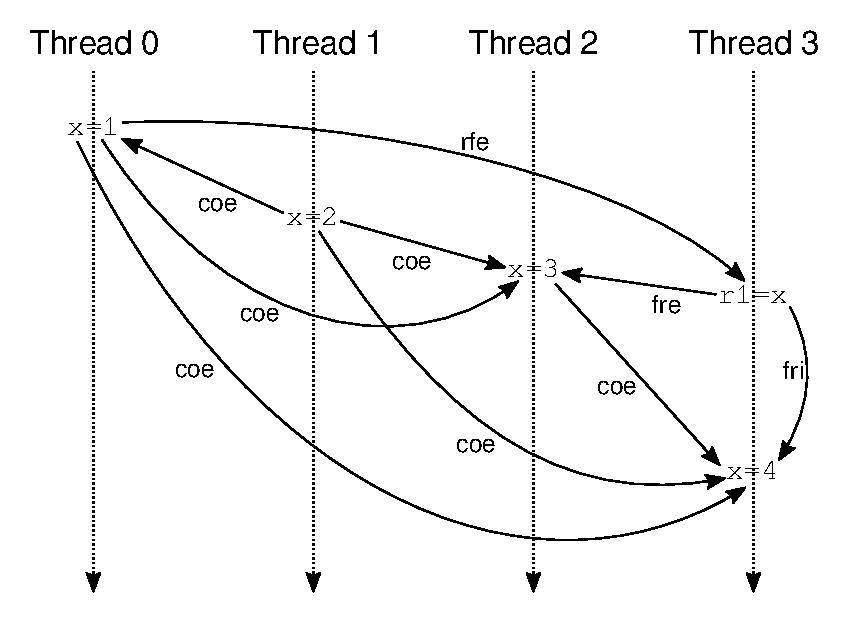
\includegraphics{ipc}}
\caption{IPC Diagram for coe, fre, and rfe}
\label{fig:IPC Diagram for coe, fre, and rfe}
\end{center}
\end{figure}

Thirdly, Figure~\ref{fig:IPC Diagram for coe, fre, and rfe} illustrates
the coe, fre, fri, and rfe links for four threads with time advancing
from the top to the bottom of the figure.  Starting with coe, even though
Thread~1's store was later in global time than that of Thread~0, that of
Thread~1 came first in coe order, followed by those of Threads~2 and ~3.
There is thus a coe link from Thread~1's store to every other store,
from Thread~0's store to those of Threads~2 and~3, and from Thread~2's
store to that of Thread~3.
This situation can occur due to the initial placement and subsequent
movement of cache lines.

Thread~3's load reads the value stored by Thread~0's store, so there is
an rfe link from that store to that load.  There is also an fre link from
that load to Thread~2's store and an fri link to Thread~3's later store.
Note that this fre link goes backwards in time.

Finally, there might be a desire for hard evidence that coe and fre
links really can go backwards in time.
We provide this evidence on x86 to demonstrate that these effects
are not confined to weakly ordered systems.
This system is a laptop with Intel(R) Core(TM) i9-10885H CPU @ 2.40GHz,
having a single socket with 8~cores, each having a pair of hardware
threads.
The code generating this data may be found in the \path{CodeSamples/cpu}
directory of the
perfbook~\cite{McKenney2018ParallelProgramming-2018-12-08a}.\footnote{
	\co{git clone git://git.kernel.org/pub/scm/linux/kernel/git/paulmck/perfbook.git}}

\begin{figure}[tb]
\begin{center}
\resizebox{3in}{!}{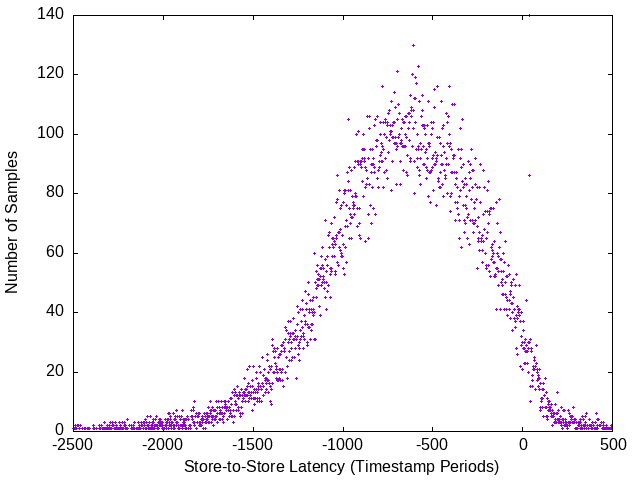
\includegraphics{coe-sh-out}}
\caption{On x86, coe Links Are Atemporal}
\label{fig:On x86, coe Links Are Atemporal}
\end{center}
\end{figure}

Figure~\ref{fig:On x86, coe Links Are Atemporal}
shows the results of 15 of the laptop's hardware threads simultaneously
storing their identifying integer (ranging from 0 to 14) to a shared
variable, then repeatedly doing timestamped reads from that variable.
The x-axis displays time in TSC periods, each of which is about 0.417~ns
in duration.
The y-axis shows the number of distinct opinions that the hardware
threads have as a function of time, a number that is frequently rather
larger than one.
The backwards-in-time coe link from Thread~1 to Thread~0 in
Figure~\ref{fig:IPC Diagram for coe, fre, and rfe}
is therefore entirely plausible.

\begin{figure}[tb]
\begin{center}
\resizebox{5in}{!}{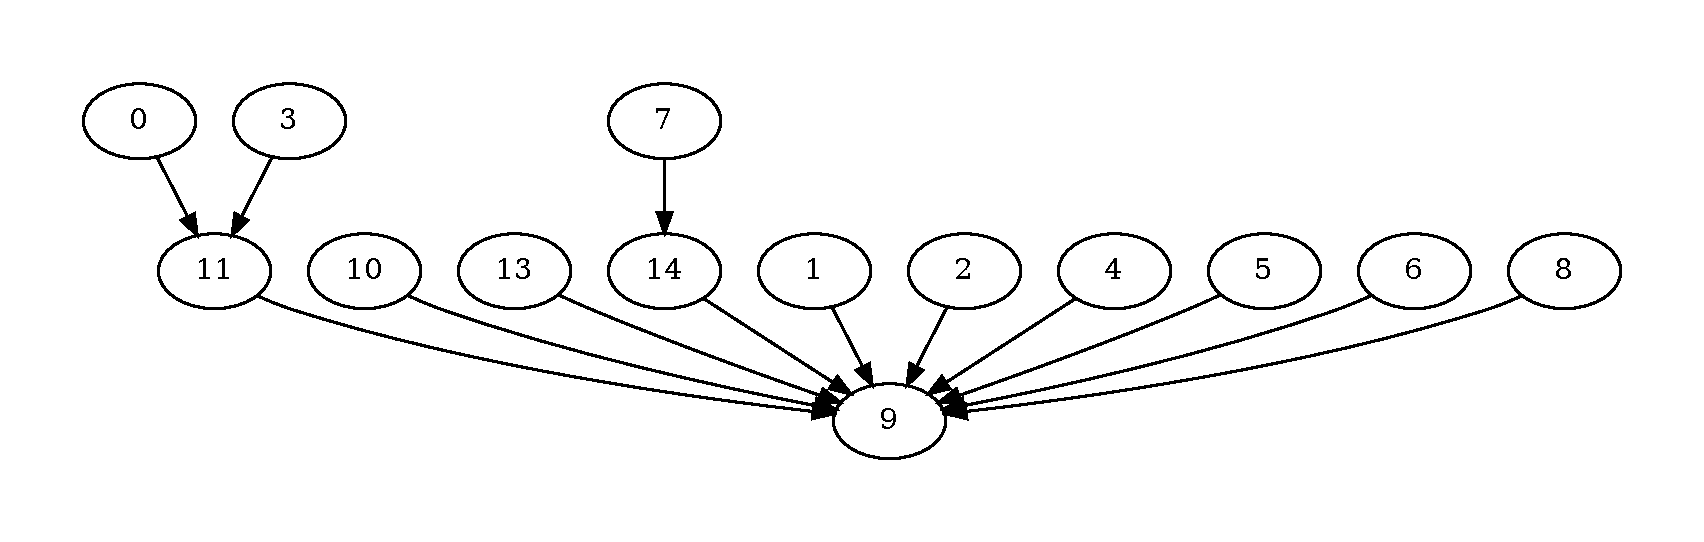
\includegraphics{coe-out-1}}
\caption{On x86, coe Links Are Partially Ordered}
\label{fig:On x86, coe Links Are Partially Ordered}
\end{center}
\end{figure}

\begin{figure}[tb]
\begin{center}
\resizebox{3in}{!}{\rotatebox{90}{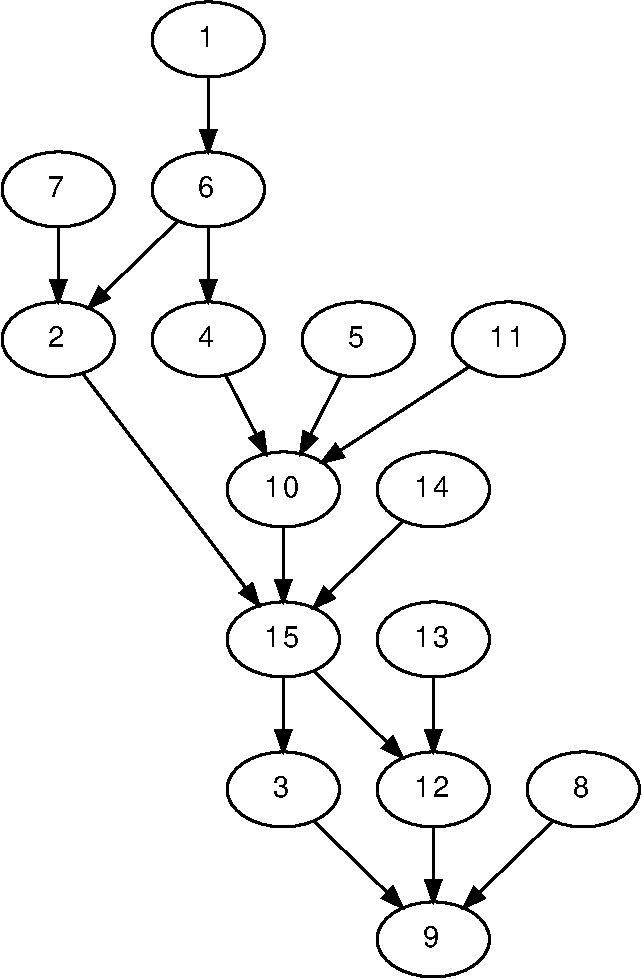
\includegraphics{store15tred}}}
\caption{On Power5, coe Links Are Also Partially Ordered}
\label{fig:On Power5, coe Links Are Also Partially Ordered}
\end{center}
\end{figure}

However, Figure~\ref{fig:On x86, coe Links Are Partially Ordered}
shows that the order of reads of each value at each thread are
consistent with a number of global orders, as required.
Figure~\ref{fig:On Power5, coe Links Are Also Partially Ordered}
shows a rather more elaborate partial order from a Power5
system~\cite{McKenney2018ParallelProgramming-2018-12-08a}.

\begin{figure}[tb]
\begin{center}
\resizebox{3in}{!}{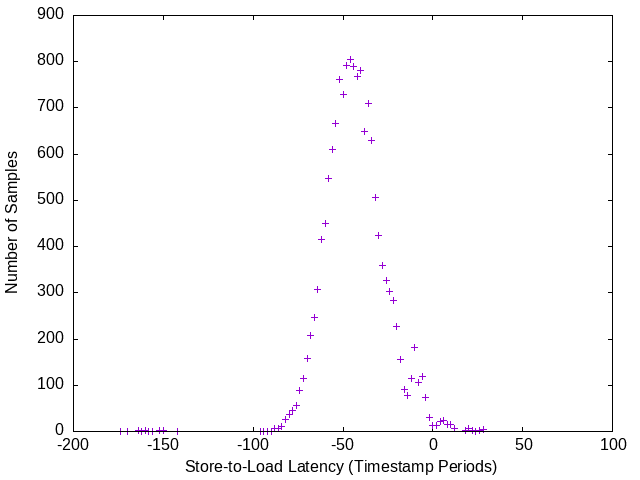
\includegraphics{fre-sh-out}}
\caption{On x86, fre Links Are Atemporal}
\label{fig:On x86, fre Links Are Atemporal}
\end{center}
\end{figure}

Figure~\ref{fig:On x86, fre Links Are Atemporal}
plots a histogram of the elapsed time from the last load to return the
old value to the store that provided the new value.
Note well that most of the data falls into negative time, that is to say,
the last load of the old value executes about 50 timestamp periods (about
20~nanoseconds) \emph{after} the store that overwrote that same old value.
That is, fre links can and do go backwards in time.
This corresponds to the fre link between Thread~3 and Thread~2 depicted in
Figure~\ref{fig:IPC Diagram for coe, fre, and rfe}.

\begin{figure}[tb]
\begin{center}
\resizebox{3in}{!}{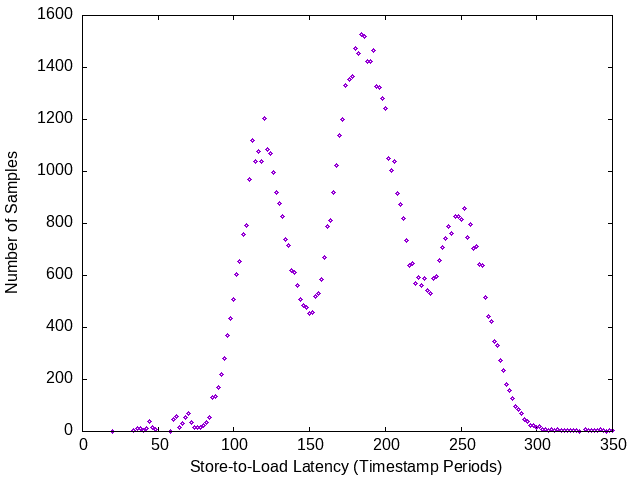
\includegraphics{rfe-sh-out}}
\caption{On x86, rfe Links Are Temporal}
\label{fig:On x86, rfe Links Are Temporal}
\end{center}
\end{figure}

Figure~\ref{fig:On x86, rfe Links Are Temporal}
plots a histogram of the elapsed time from a store of a new value
to the first load of that new value.
Note well that all of the data falls into positive time, indicating
that rfe links always go forward in time, as those familiar with
computer hardware and the laws of physics would expect.

\begin{figure}[tb]
\begin{center}
\resizebox{4in}{!}{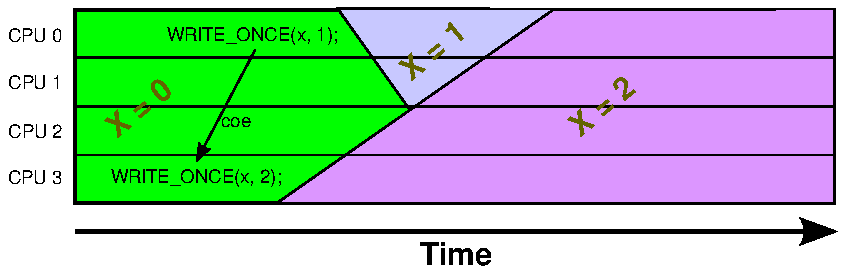
\includegraphics{coe}}
\resizebox{4in}{!}{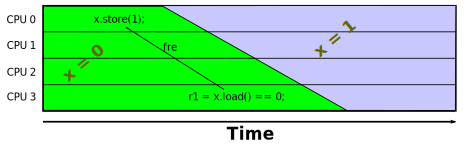
\includegraphics{fre}}
\resizebox{4in}{!}{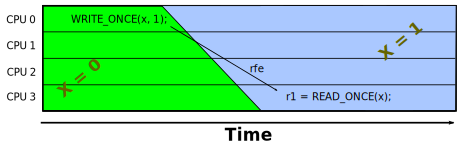
\includegraphics{rfe}}
\caption{Propagation Delay and Temporal Properties of coe, fre, and rfe}
\label{fig:Propagation Delay and Temporal Properties of coe, fre, and rfe}
\end{center}
\end{figure}

Figure~\ref{fig:Propagation Delay and Temporal Properties of coe, fre, and rfe}
shows how the temporal properties of coe, fre, and rfe are explained
by propagation delay.
In the case of coe, the two stores take time to propagate across the
system, and their ordering can be and often is decided after the fact.
In the case of fre, the store again takes time to propagate across
the system, and so a load might execute later in global time than
did the store, but not late enough to return that store's value.
In the case of rfe, the load cannot return a given store's value until
the value has propagated to that part of the system executing that load.

And this is exactly why the C++ memory model guarantees ordering from
rfe links but not the coe and fre links for relaxed accesses in the
absence of other ordering from stronger atomic memory accesses or
\co{atomic_thread_fence(memory_order_seq_cst}.

\clearpage

\section{User Influence Over Language Semantics}
\label{app:User Influence Over Language Semantics}

As noted earlier, the exact definition of a computer language is subject
to some debate, with standards, implementations, and users all having
some degree of
influence~\cite{KayvanMemarian2016DepthOfC-1,KayvanMemarian2016DepthOfC-2},
and each of which is subject to change over time.
It is natural to dismiss user influence when compared to the text of
standards or the code in implementations, but both are subject to
change and do change over time.
The implementation is especially subject to change, for example,
consider the following command line used to build the Linux kernel's
\co{kernel/rcu/tree.c} C-language source file:

~\\
{
	\scriptsize
	\texttt{
	gcc -Wp,-MMD,kernel/rcu/.tree.o.d -nostdinc
	-I./arch/x86/include \\
	-I./arch/x86/include/generated  -I./include
	-I./arch/x86/include/uapi \\
	-I./arch/x86/include/generated/uapi
	-I./include/uapi -I./include/generated/uapi \\
	-include ./include/linux/compiler-version.h
	-include ./include/linux/kconfig.h \\
	-include ./include/linux/compiler\_types.h -D\_\_KERNEL\_\_
	-fmacro-prefix-map=./= \\
	-Werror -std=gnu11 -fshort-wchar
	-funsigned-char -fno-common -fno-PIE \\
	-fno-strict-aliasing -mno-sse
	-mno-mmx -mno-sse2 -mno-3dnow -mno-avx \\
	-fcf-protection=branch
	-fno-jump-tables -m64 -falign-jumps=1 -falign-loops=1 \\
	-mno-80387 -mno-fp-ret-in-387 -mpreferred-stack-boundary=3
	-mskip-rax-setup \\
	-mtune=generic -mno-red-zone -mcmodel=kernel
	-Wno-sign-compare \\
	-fno-asynchronous-unwind-tables
	-mindirect-branch=thunk-extern \\
	-mindirect-branch-register
	-mindirect-branch-cs-prefix -mfunction-return=thunk-extern
	-fno-jump-tables -fpatchable-function-entry=16,16
	-fno-delete-null-pointer-checks -O2 \\
	-fno-allow-store-data-races
	-fstack-protector-strong -fomit-frame-pointer \\
	-fno-stack-clash-protection -falign-functions=16
	-fno-strict-overflow -fno-stack-check \\
	-fconserve-stack
	-Wall -Wundef -Werror=implicit-function-declaration \\
	-Werror=implicit-int -Werror=return-type -Werror=strict-prototypes \\
	-Wno-format-security -Wno-trigraphs -Wno-frame-address
	-Wno-address-of-packed-member \\
	-Wframe-larger-than=2048 -Wno-main
	-Wno-unused-but-set-variable \\
	-Wno-unused-const-variable -Wvla
	-Wno-pointer-sign -Wcast-function-type \\
	-Wno-array-bounds
	-Wno-alloc-size-larger-than -Wimplicit-fallthrough=5 \\
	-Werror=date-time -Werror=incompatible-pointer-types
	-Werror=designated-init \\
	-Wenum-conversion
	-Wno-unused-but-set-variable -Wno-unused-const-variable \\
	-Wno-restrict -Wno-packed-not-aligned -Wno-format-overflow
	-Wno-format-truncation \\
	-Wno-stringop-overflow
	-Wno-stringop-truncation -Wno-missing-field-initializers \\
	-Wno-type-limits -Wno-shift-negative-value
	-Wno-maybe-uninitialized \\
	-Wno-sign-compare
	-DKBUILD\_MODFILE='"kernel/rcu/tree"'
	-DKBUILD\_BASENAME='"tree"' \\
	-DKBUILD\_MODNAME='"tree"' -D\_\_KBUILD\_MODNAME=kmod\_tree \\
	-c -o kernel/rcu/tree.o kernel/rcu/tree.c
	}
}

We do not propose to explain all of these, and sufficiently motivated
readers can avail themselves of the GCC documentation.
We instead look at representative members of several categories.

The \co{-funsigned-char} causes type \co{char} to be unsigned, which
overrides per-architecture defaults, some of which treat \co{char}
as signed and others as \co{unsigned}.
This choice prevents a class of bugs, and also allows the kernel to make
reliable use of the uppermost bit of variables of type \co{char}.
It also affects the definition of ``semantic dependency'' by changing
the arithmetic proporties of this type.
In theory, the standard could specify the signedness of \co{char}, but the
variety of existing practice in the 1980s prevented this.
Plus machine instructions were much more expensive back then, so the
signedness of \co{char} was much more of a performance concern than
it is toda than
it is todayy.

The \co{-mno-sse} prevents GCC from making use of the SSE hardware.
This is done for performance reasons, as it avoids the overhead of
saving and restoring the state of this hardware when switching between
user and kernel contexts.
Similarly, the \co{-mcmodel=kernel} causes the kernel binary to be
placed in the uppermost 2GB of the address space, again reducing
the overhead of switching between user and kernel contexts.
These are cases where the standard does not specify anything, nor
should it.

The \co{-fpatchable-function-entry=16,16} causes GCC to emit 16
\co{nop} instructions at the beginning of each function, with
the function's entry point being just after this string of \co{nop}
instructions.
The resulting buffers are used by the Linux-kernel tracing infrastructure
which is in turn used for debugging, performance measurement, and
monitoring.
This is again clearly outside of the scope of the standard.

The \co{-fstack-protector-strong} causes GCC to emit code that provides
some protection against some clases of attacks based on buffer overflows.
One could rightly argue code should simply avoid ever overflowing buffers,
but things like memory allocators and userspace memory accesses must
use code that can be difficult to distinguish from buffer overflows.
It is not clear that the ever-increasing variety of attacks should
affect the standard.

The \co{-fno-strict-overflow} causes GCC to act as if signed integer
overflow is defined behavior.
Note well that this command-line option also affects the definition of
``semantic dependency''.
This might be a controversial choice, and another option would be to add
a new set of signed integer types to the standard for which overflow is
defined as wrapping, similar to the situation with unsigned integers.

The \co{-Werror=strict-prototypes} causes GCC to warn if old-style
non-ANSI function prototypes are used.
This helps avoid certain classes of bugs.
Warnings are by design outside of the scope of the standard.

In other words, user preference can exert a non-trivial influence over
language semantics, and in particular can affect some aspects of the
definition of ``semantic dependency''.

\clearpage

\section{Debates on Causality}
\label{sec:Debates on Causality}

This Appendix is provided as a service to readers who want to know more
about the ongoing debates on causality, provided by the combined efforts
of Bard, Chat-GPT, and Bing Co-Pilot.
References may be found here:

{ \scriptsize
\url{https://docs.google.com/document/d/1MJ6pQ4TcWchUQvoI-qhLjdhPVYF14AytbTW3gr4-xag/edit?usp=sharing}
}

The concept of causality, the idea that events are caused by preceding
events in a predictable and consistent manner, is fundamental to many
scientific theories and our understanding of the world.
However, when it comes to the universe as a whole, particularly at the
most fundamental levels such as in quantum physics or the origins of
the universe, the idea of strict causality can become more complex.

In classical physics, causality is often described in terms of
deterministic laws, where events are determined by prior causes.
But at the quantum level, the behavior of particles can be probabilistic
and uncertain.
Quantum mechanics introduces a level of randomness and uncertainty that
challenges our classical notions of causality.

Additionally, when considering the origin of the universe (the Big Bang),
the laws of physics as we understand them break down at extremely high
densities and temperatures.
The conditions at the very beginning of the universe might not conform
to our classical understanding of causality, and some theories suggest
that time itself might have begun with the Big Bang, making it difficult
to define causality in a traditional sense within such a framework.

On the one hand, there is a strong case to be made that the universe
is causal.
Our understanding of physics is based on the principle of causality,
which states that every event has a cause.
This principle has been incredibly successful in explaining and predicting
the behavior of the universe at large scales.
Additionally, our own personal experience seems to confirm causality.
We constantly observe events being caused by other events, and we have
no reason to believe that this is an illusion.

However, there are also some challenges to the idea of a perfectly
causal universe.
One challenge comes from quantum mechanics, which suggests that some
events may be fundamentally non-causal.
For example, the collapse of a wave function in quantum mechanics seems
to be a random event, with no underlying cause.
Additionally, our understanding of the universe's origins is still
very limited.
We don't know whether the Big Bang itself had a cause, or whether it
was simply the beginning of everything.

In summary, while causality is a fundamental concept in our understanding
of the universe, its application and implications can become more complex,
especially at the quantum level and regarding the origin of the universe.
There are ongoing debates and explorations within physics and philosophy
about the nature of causality in these contexts.

% \section{History}
% \label{sec:History}

\clearpage

\section{Acknowledgments}
\label{sec:Acknowledgments}

We are grateful to David Goldblatt, Jade Alglave, and Peter
Sewell for their careful review of an early draft of this paper and
to John Wickerson for asking Paul for a rant and taking the proffered
rant seriously.
We also owe David Goldblatt a debt of gratitude for his having asked an
insightful question at the right time, his insights on combinations of
OOTA and UB, and for his ``Deathstation 9000'' demonic CPU.
% Alan Stern located many unclear statements and gaps in reasoning.
Martin Uecker contributed valuable insights on backwards-propagating UB.
Richard Grisenthwaite patiently explained the architectural constraints
that prevent hardware OOTA.

Nonetheless, all errors and omissions in this paper are the sole property
of the authors, and the appearance of a name in this appendix does
not in any way constitute agreement with anything in this paper.

% @@@ reviewer to do.
% Luc Maranget: Memory models.
% Greg Kroah-Hartman and Linus Torvalds: FYI, trouble being caused.
% Christoph Hellwig: Why slow on BPF memory model.
% Miguel Ojeda: LKMM and Rust.
% Alice Ryhl: LKMM and Rust.
% Ralf Jung: Rust.
% Catalin Marinas: ARM and formal methods (qspinlock).
% Segher Boessenkool:  GCC.
% Dan Lustig: NVIDIA memory ordering.
% Andrea Parri: Memory models, RISC-V hardware.
% Jonas Oberhauser: Memory models.
% Hernan Ponce de Leon: Memory models.
% Palmer Dabbelt: RISC-V hardware.
% Ali Sezgin: P0422R0.
% Tony Tye: P0422R0.
% Other memory-model maintainers.
% Derek Williams: PowerPC hardware.
% Hans Boehm: Skeptic, memory models, OOTA.  Suggestions for others?
% Olivier Giroux: Skeptic, memory models, NVIDIA.
% Luke Geeson: Whatever...  Review.
% Ori Lahav: Prior OOTA.
% Viktor Vafeiadis:  Prior OOTA.
% Derek Dreyer: Prior OOTA.
% Brian Demsky: Prior OOTA.

% Done as of December 18, 2023:
% David Goldblatt
% Boqun Feng, Uladzislau Rezki, Neeraj Upadhyay, Joel Fernandes, and
%	Frederic Weisbecker (RCU proteges)
% Michael Wong
% Maged Michael
% John Wickerson: Thank you.  OK for Peter Sewell, Mark Batty, etc.
% Akira Yokosawa: Professional courtesy, perfbook memory models.
% Dan Kelley, Alexei Starovoitov, Mykola Lysenko: FYI.  OOTA dropped
% Alan Jeffrey: Fixed-point insight P0422R0.  Reached out via LinkedIn.
% Jade Alglave: C++ herd model?  Memory models and variety of hardware.
% Alan Stern: Memory models, mathematical logic, and variety of hardware.
% Martin Uecker (offered)
% Peter Sewell
% Mark Batty
% Richard Gristenthwaite: ARM hardware.  Posed HW speculation question.
% Peter Zijlstra.
% Mark Rutland: ARM memory ordering.
% Will Deacon: ARM hardware, C++, and OOTA.

% @@@ TODO:
% Create nice bell graph for coe, or at least try!
% Construct interleaved OOTA examples (see sheets of paper).
% Check cmbc on nondeterministic i++.
% Use LKMM as check for dependencies?

% Objections:
% "Atomic operations are not observable behavior."
%	They are for volatile atomic objects.  Plus an implementation
%	whose analysis is confined to a thread would need to assume
%	that any atomic store might lead to observable behavior in some
%	other thread.  An implementation with a global view must preserve
%	observable behavior regardless of OOTA cycles.	Plus if an OOTA
%	cycle does not affect observable behavior, who cares?
% "The C++ abstract machine is independent of the laws of physics."
%	That might be, but any real implementation of that abstract
%	machine will be governed by those laws.
% "Real hardware can exhibit OOTA, as exemplified by audio feedback."
%	Such hardware does not run C++.  Also, audio feedback is more
%	closely approximated by a loop calculating sound intensity than
%	by OOTA, especially given that you must include the audio
%	properties of the enclosing space in analyzing the feedback loop.

% Additional snark:
% "This work reduces the problem of OOTA analysis to that of sequential
%	program analysis.  If you expect better verification of concurrent
%	code than of sequential code, you are in an intellectual state
%	of sin."
% "Forcing relaxed loads to be ordered before subsequent relaxed stores
%	is an expensive no-op."
% "So you don't want to learn concurrency?  Then I can only suggest
%	that you either move further up the stack or take early
%	retirement."  Note that that C++ committee's concurrency
%	expertise has grown beyond recognition over the past 15 years.

% One-pager:
% Threats to validity:
% Speed of light might not always be finite.
% Zero-sized atoms might be discovered.
% It might be possible to propagate information at infinite velocity
%	despite the finite speed of light.
% It might be possible to violate causality.
% Hardware and compiler bugs might result in OOTA.
% ML hallucination might convince people that OOTA is OK.

\bibliographystyle{plain}
\bibliography{bib/RCU,bib/WFS,bib/hw,bib/os,bib/parallelsys,bib/patterns,bib/perfmeas,bib/refs,bib/syncrefs,bib/search,bib/swtools,bib/realtime,bib/TM,bib/standards,bib/memorymodel.bib}

\end{document}
